\documentclass[aspectratio=169]{beamer}
%\documentclass[aspectratio=43]{beamer}
%\documentclass[newPxFont,sthlmFooter]{beamer}
\usetheme{sthlm}
%\usecolortheme{sthlmv42}

%-=-=-=-=-=-=-=-=-=-=-=-=-=-=-=-=-=-=-=-=-=-=-=-=
%        LOADING PACKAGES
%-=-=-=-=-=-=-=-=-=-=-=-=-=-=-=-=-=-=-=-=-=-=-=-=
\usepackage[utf8]{inputenc}
\usepackage{lscape}
\usepackage{tikz}
\usepackage{marvosym}
\usepackage{chronology}
\usepackage[english]{babel}
\definecolor{airforceblue}{rgb}{0.2,0.2,0.7}
\usepackage{xcolor}
\usepackage{float}
\usepackage{cancel}
%\spanishdecimal{.}
\renewcommand{\event}[3][e]{%
  \pgfmathsetlength\xstop{(#2-\theyearstart)*\unit}%
  \ifx #1e%
    \draw[fill=black,draw=none,opacity=0.5]%
      (\xstop, 0) circle (.2\unit)%
      node[opacity=1,rotate=45,right=.2\unit] {#3};%
  \else%
    \pgfmathsetlength\xstart{(#1-\theyearstart)*\unit}%
    \draw[fill=black,draw=none,opacity=0.5,rounded corners=.1\unit]%
      (\xstart,-.1\unit) rectangle%
      node[opacity=1,rotate=45,right=.2\unit] {#3} (\xstop,.1\unit);%
  \fi}%

%Dirección de la imágenes
\graphicspath{ {images/} }



\newtheorem{teo}[theorem]{Teorema}
\newtheorem{definicion}[theorem]{Definici\'on}
\newtheorem{lema}[theorem]{Lema}
\newtheorem{coro}[theorem]{Corolario}
\newtheorem{propo}[theorem]{Proposici\'on}
\newtheorem{remarks}[theorem]{Notas}
\newtheorem{remark}[theorem]{Nota}
\newtheorem{claim}[theorem]{Afirmaci\'on}
%\newtheorem{examples}[theorem]{Ejemplos}
%\newtheorem{algorithm}{Algoritmo}[section]
\newtheorem{eje}[theorem]{Ejemplo}
\newtheorem{conjeture}[theorem]{Conjetura}
\newtheorem{question}[theorem]{Pregunta}
\usepackage{ulem}


\DeclareFontFamily{U}{mathx}{}
\DeclareFontShape{U}{mathx}{m}{n}{<-> mathx10}{}
\DeclareSymbolFont{mathx}{U}{mathx}{m}{n}
\DeclareMathAccent{\widehat}{0}{mathx}{"70}
\DeclareMathAccent{\widecheck}{0}{mathx}{"71}
\renewcommand{\check}{\widecheck}

%-=-=-=-=-=-=-=-=-=-=-=-=-=-=-=-=-=-=-=-=-=-=-=-=
%        BEAMER OPTIONS
%-=-=-=-=-=-=-=-=-=-=-=-=-=-=-=-=-=-=-=-=-=-=-=-=

%\setbeameroption{show notes}

%-=-=-=-=-=-=-=-=-=-=-=-=-=-=-=-=-=-=-=-=-=-=-=-=
%
%	PRESENTATION INFORMATION
%
%-=-=-=-=-=-=-=-=-=-=-=-=-=-=-=-=-=-=-=-=-=-=-=-=

\title[]{\Large\centering
\color{airforceblue}Modelo predictivo de la producción del agave en Aguascalientes: desde la siembra hasta la cosecha}
%\\


\author{{\small \textsc{presenta}}\centering{\\Isaac Vázquez Mendoza \\ {\small\textsc{
		bajo la dirección de}}\\ Dra. Magali Arellano Vázquez}}


\institute{}

\begin{document}
	\begin{frame}[noframenumbering]
		%\begin{center}
		%	\includegraphics[scale=0.5]{Encabezado.png}
		%\end{center}
		
		\begin{minipage}{0.15\textwidth}
			\centering
			\hspace{0.3cm}\vspace{-0.6cm}
\includegraphics[scale=0.23]{images/INFOTEC.jpg}
		\end{minipage}%
		\begin{minipage}{0.65\textwidth}
			\centering \vspace{0.5cm}
			\hspace{1cm}INFOTEC
			
			\hspace{1cm}Centro de Investigación e Innovación en TIC
                \hspace{1cm}
   
		\end{minipage}%
		\begin{minipage}{0.2\textwidth}
			
\includegraphics[width=.5cm]{tr.png}
                \hspace*{0.5cm}%
\includegraphics[scale=0.08]{images/EncuentroGarza.png}
		\end{minipage}
		\date{}
		\titlepage
		
		
		
	\end{frame}
%-=-=-=-=-=-=-=-=-=-=-=-=-=-=-=-=-=-=-=-=-=-=-=-=
%
%	TITLE PAGE
%
%-=-=-=-=-=-=-=-=-=-=-=-=-=-=-=-=-=-=-=-=-=-=-=-=

%\begin{frame}[plain]
%	\titlepage
%\end{frame}

%-=-=-=-=-=-=-=-=-=-=-=-=-=-=-=-=-=-=-=-=-=-=-=-=
%
%	TABLE OF CONTENTS: OVERVIEW
%
%-=-=-=-=-=-=-=-=-=-=-=-=-=-=-=-=-=-=-=-=-=-=-=-=

%\begin{frame}{Index}
%	\tableofcontents
%\end{frame}

\definecolor{mygray}{gray}{0.95}

{
	\setbeamercolor{background canvas}{bg=mygray}
	\vspace{-2cm}\begin{frame}{Mapa de contenidos}
		\begin{itemize}
			\color{airforceblue}
			\item Motivación del problema.
			\item Panorama de la industria agrícola.
			\item Impacto del cambio climático en la agricultura.
			\item El agave y Aguascalientes.
			\item Pregunta de investigación.
			\item Objetivos.
			\item Estado del arte.
			\item Factibilidad
			\item Referencias.
		\end{itemize}
	\end{frame}
}

\begin{frame}{Motivación del problema}
	\vspace{-1.5cm} \centering
	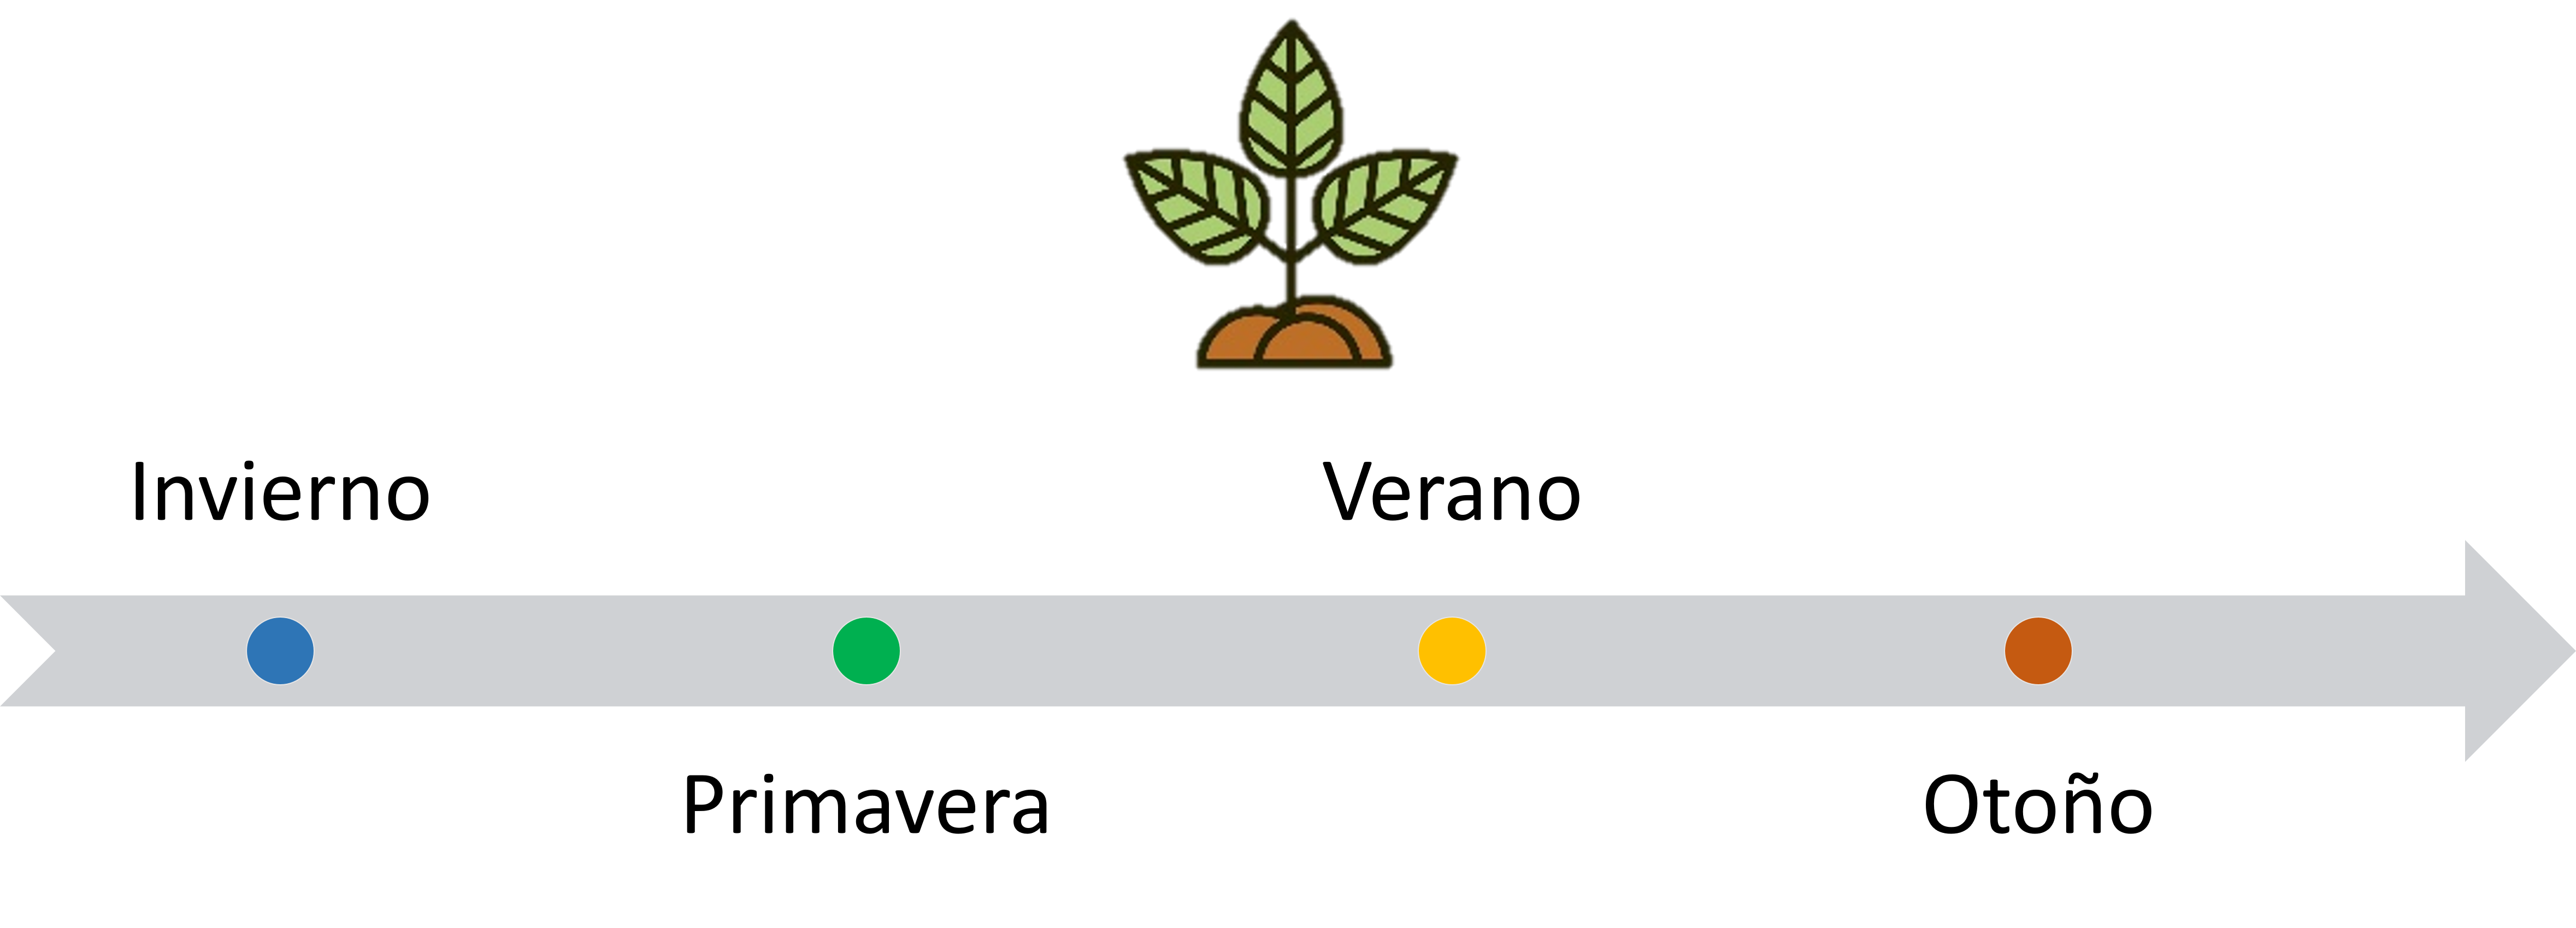
\includegraphics[width=\textwidth]{images/Choice.png}
\end{frame}

\begin{frame}{Motivación del problema}
	\vspace{-1cm}\centering
	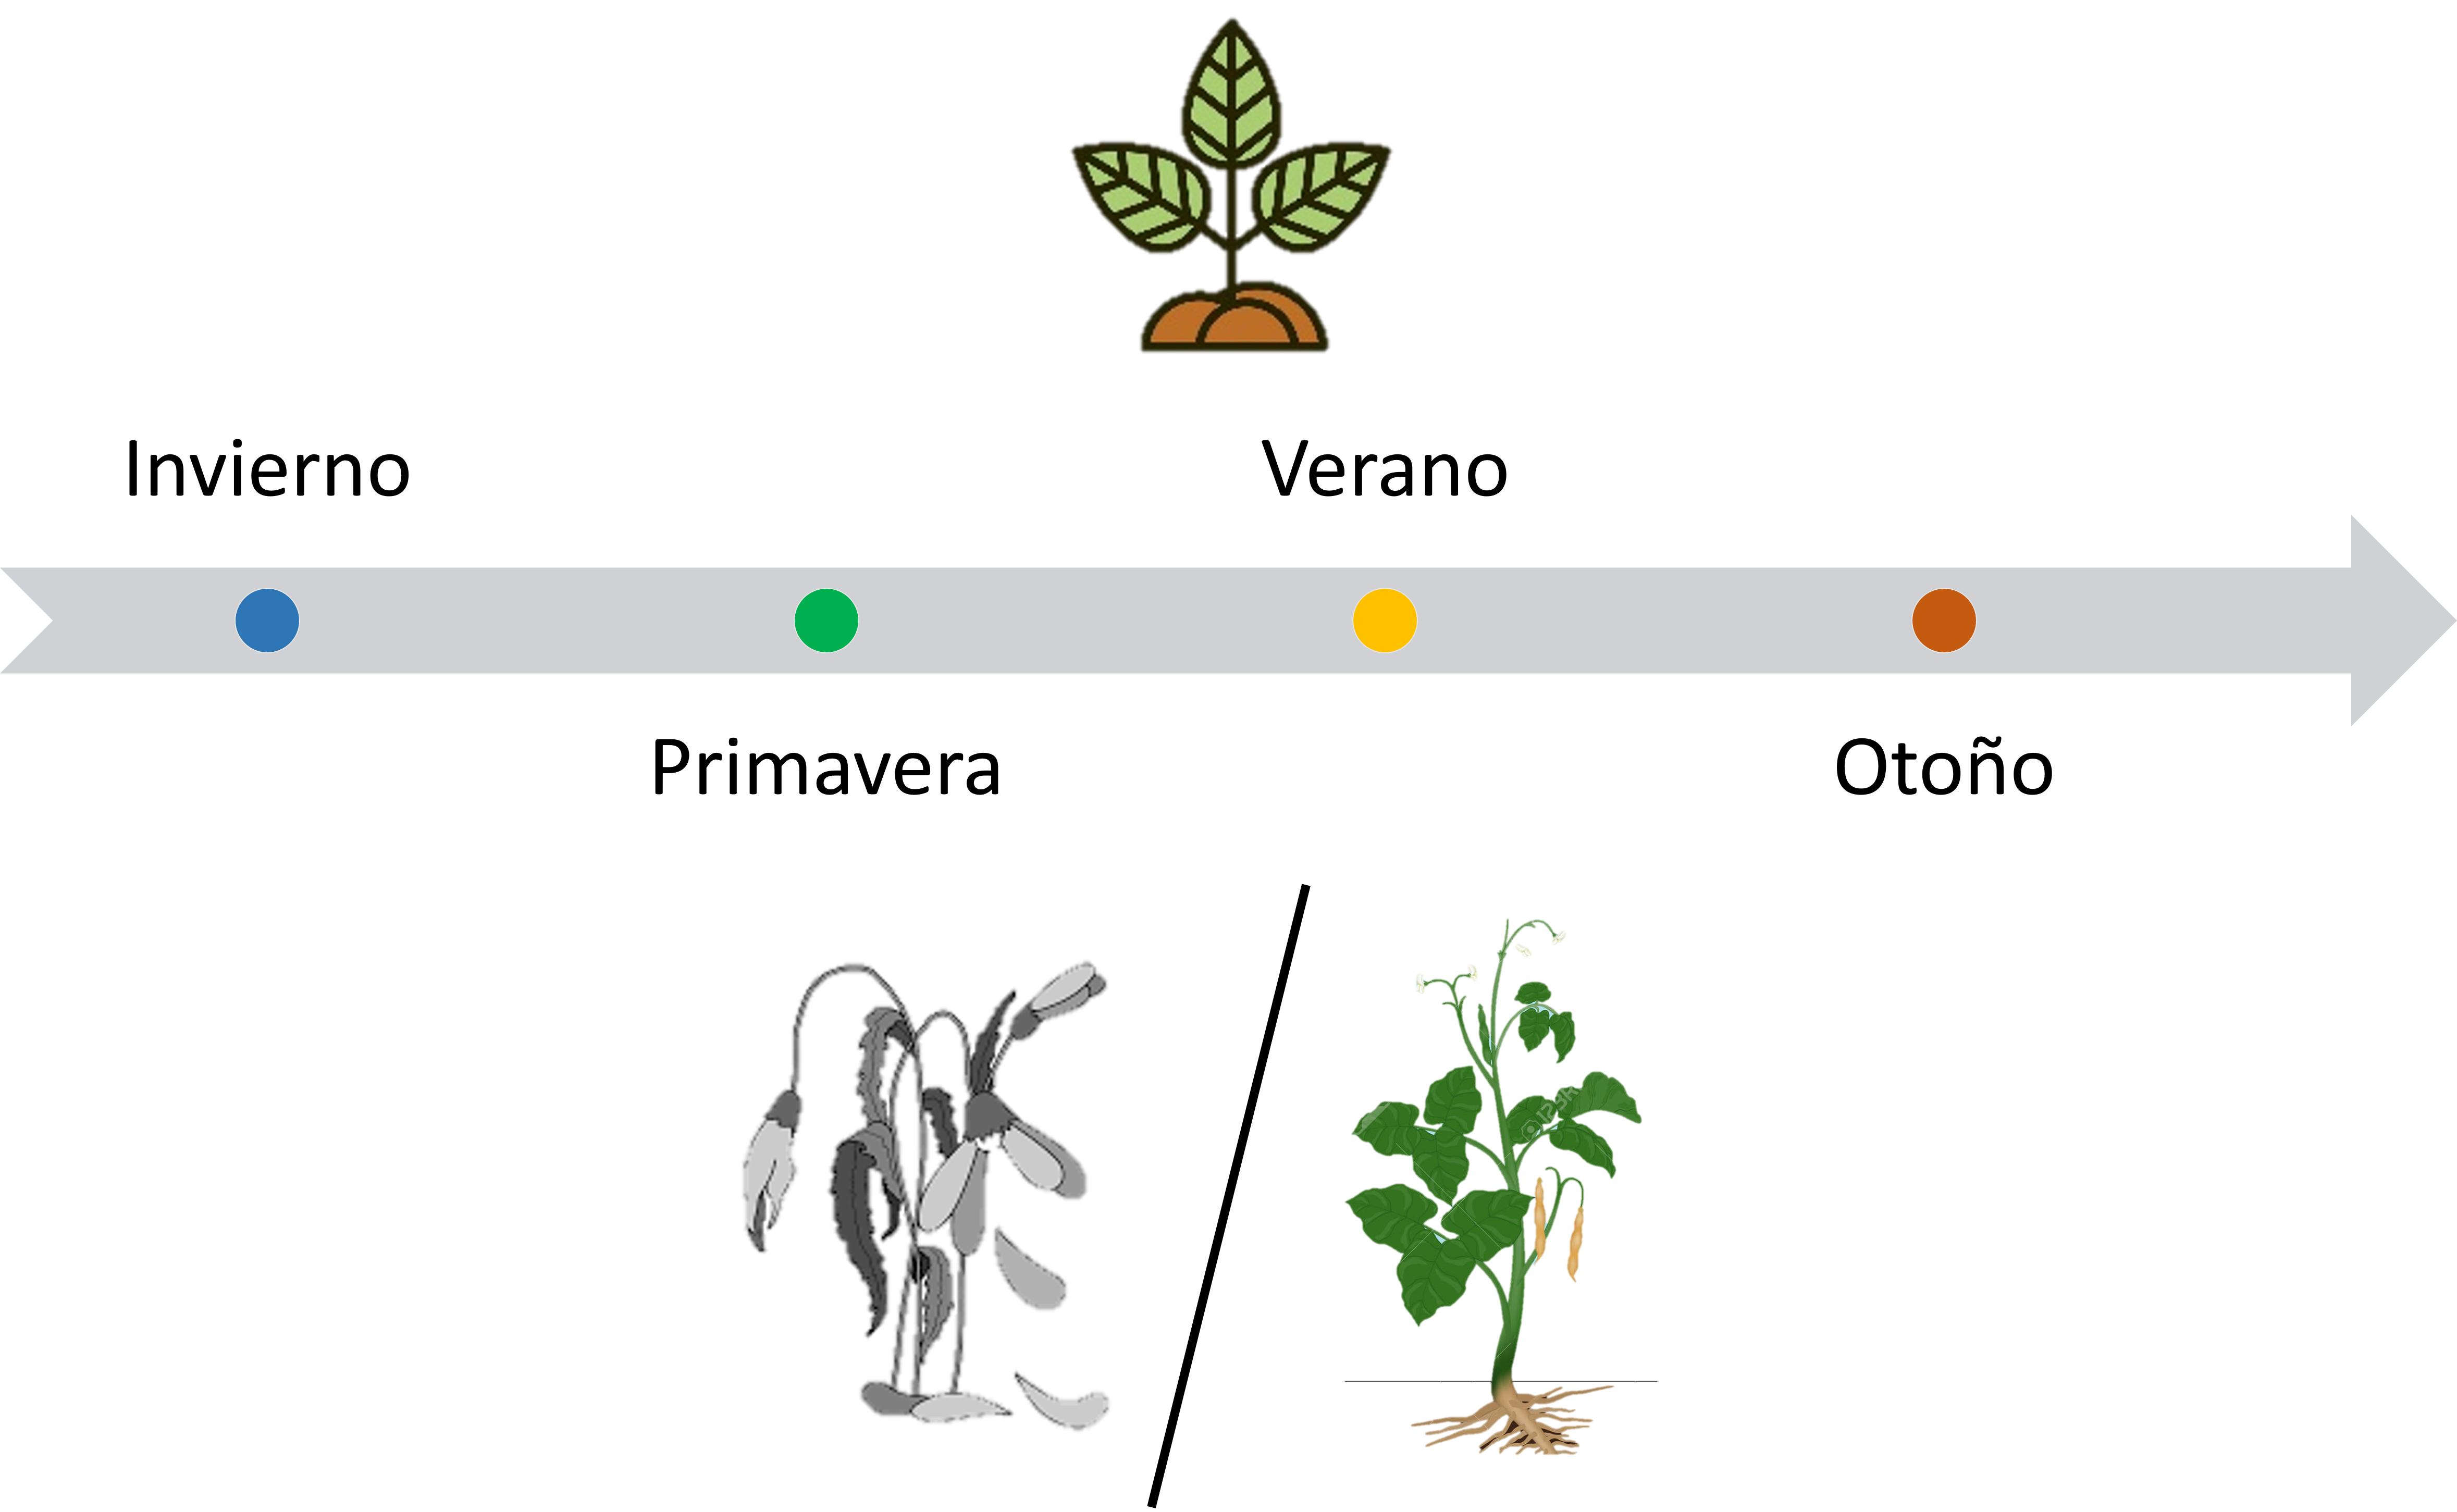
\includegraphics[width=0.9\textwidth]{images/Survival.png}
\end{frame}

\begin{frame}{Motivación del problema}
	 \vspace{-1cm}
	 \centering
	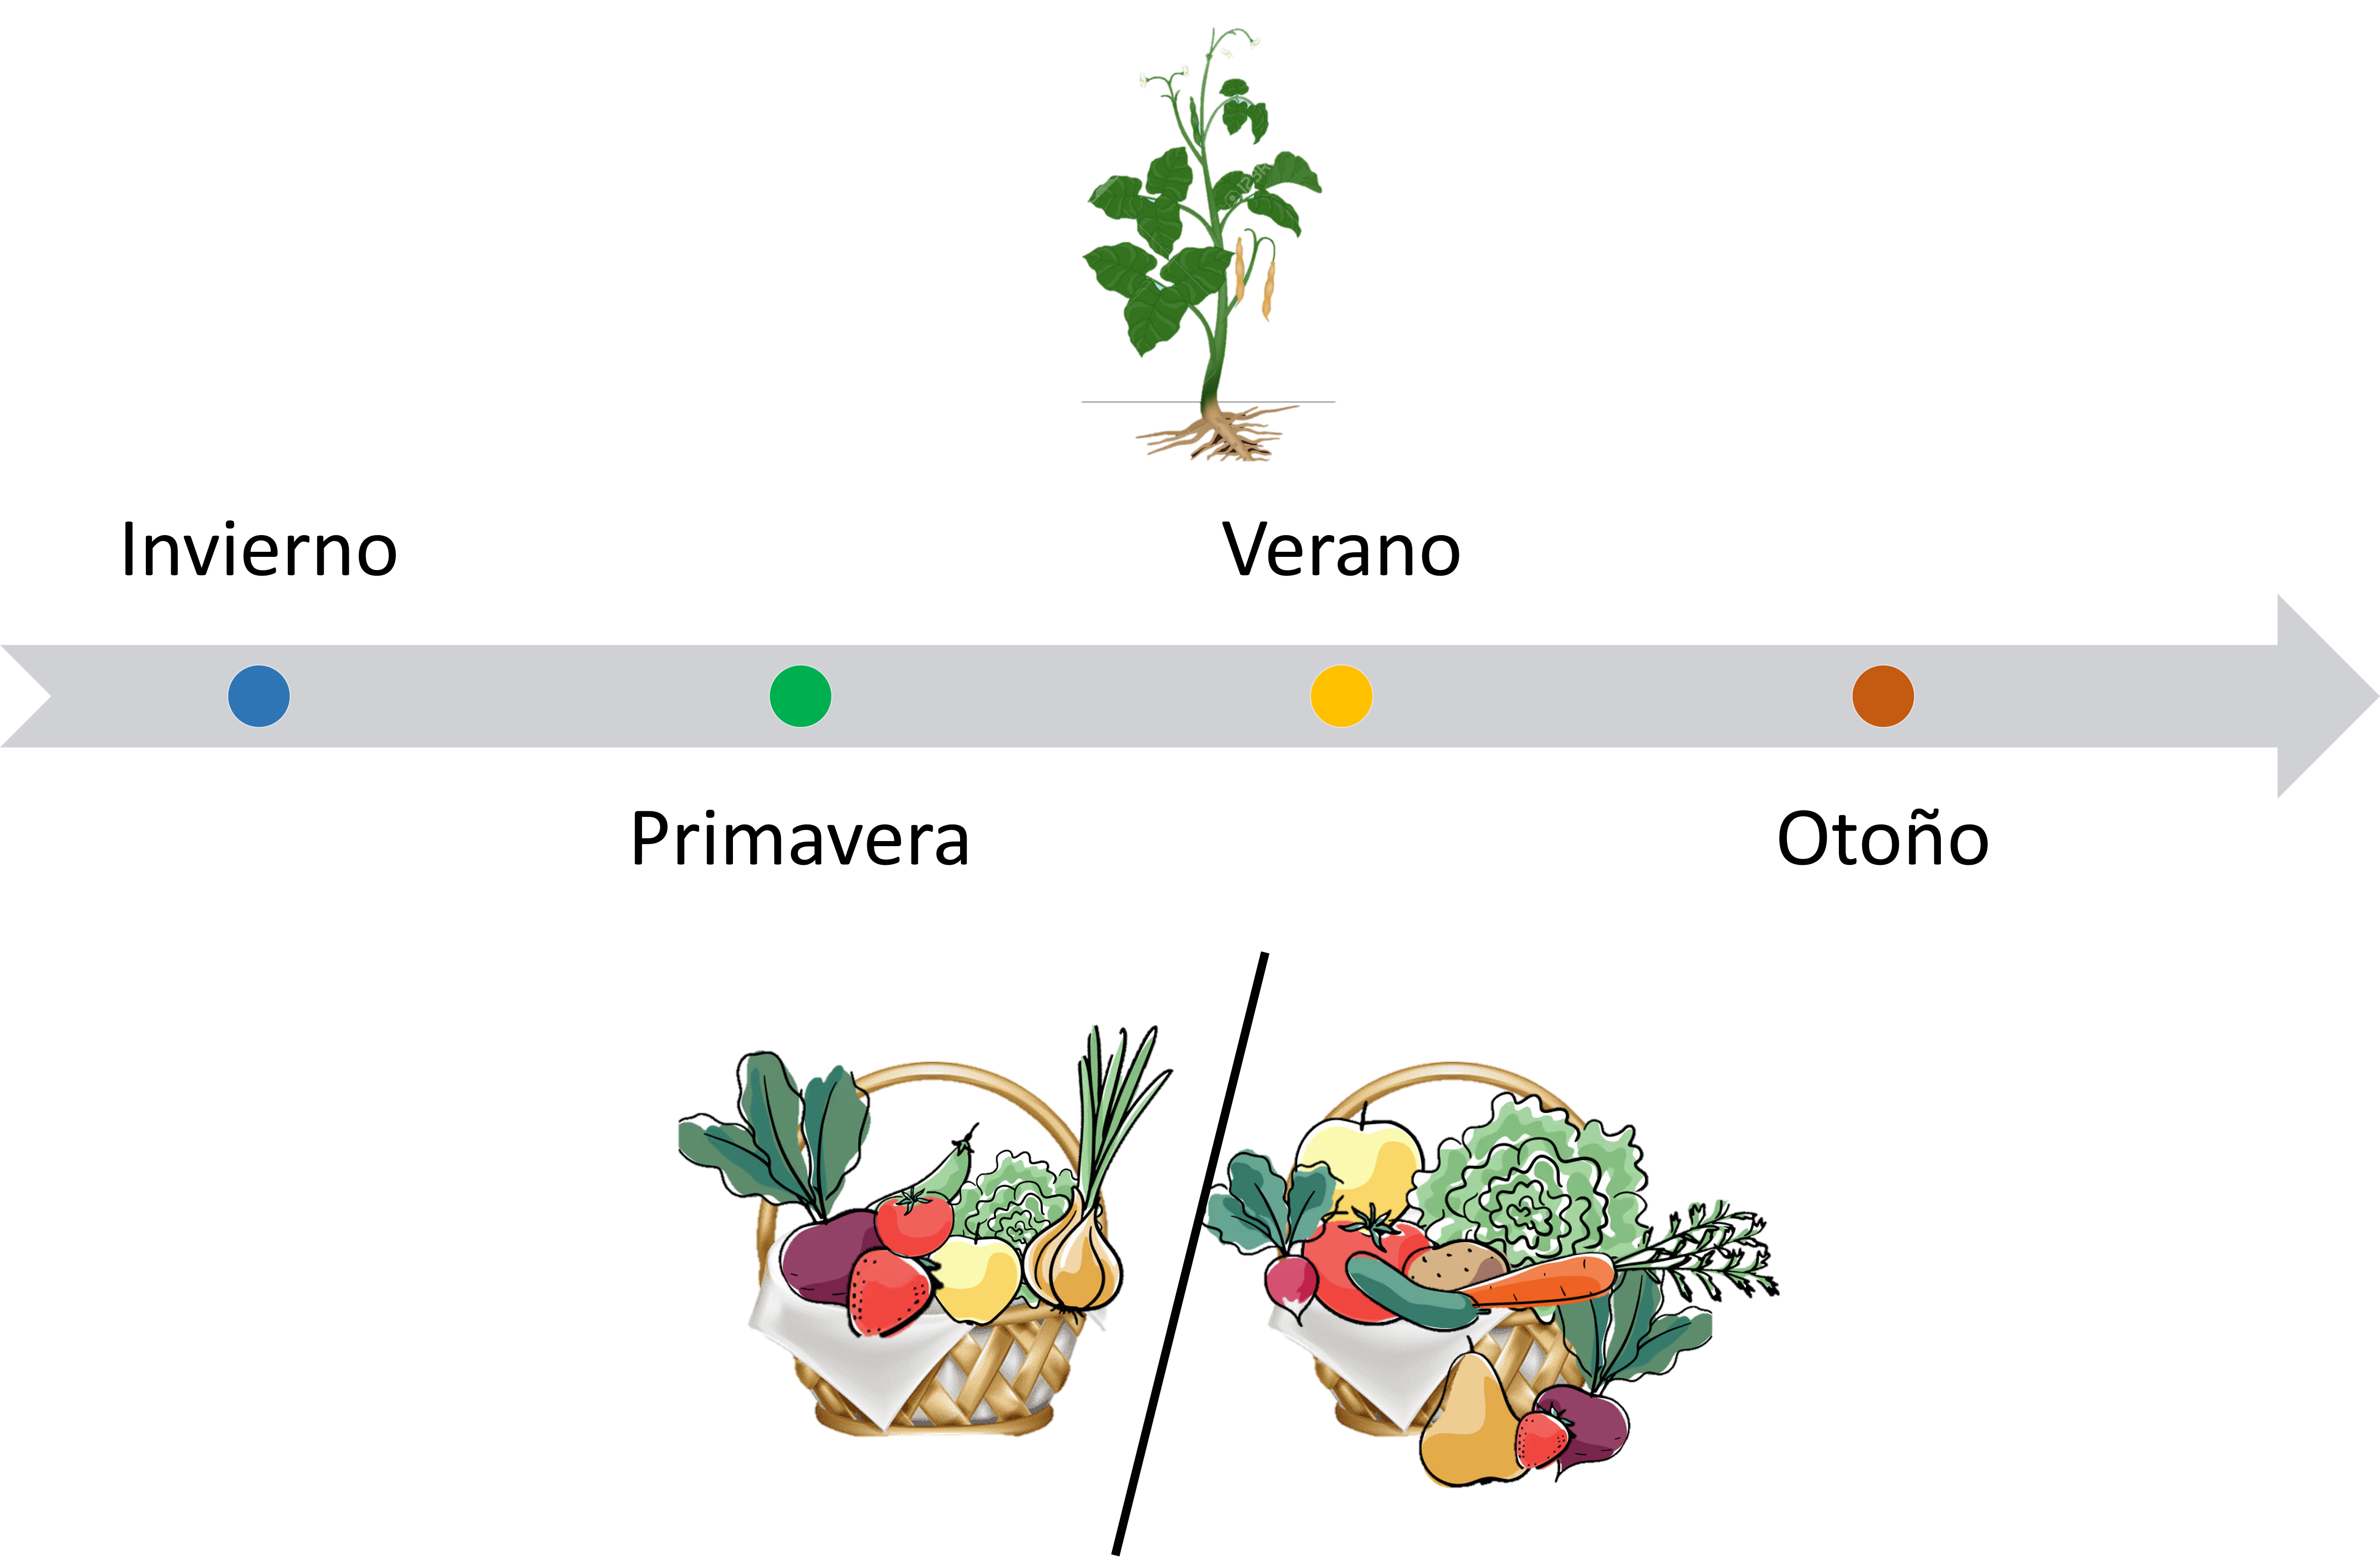
\includegraphics[width=0.9\textwidth]{images/Production.png}
\end{frame}


\begin{frame}{Motivación del problema}
\begin{block}{\centering Proceso de decisión}
	\begin{minipage}{0.5\textwidth}
		\pause\begin{itemize}
			\item Conocimiento ancentral.
			\item Sistematización y mecanización.
			\item Estudios científicos.
			\item Interacciones multidisciplinarias.
		\end{itemize}
	\end{minipage}%
	\begin{minipage}{0.5\textwidth}
			 \phantom{text}
			\phantom{text}
			\phantom{text}
			\phantom{text}
	\end{minipage}
\end{block}
\centering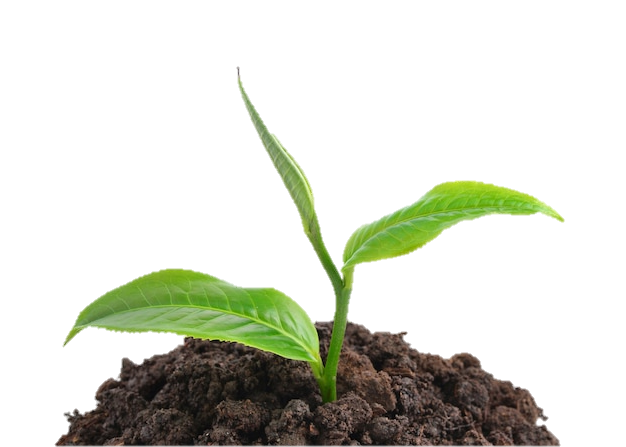
\includegraphics[width=0.4\textwidth]{images/Agro.png}
\end{frame}

\begin{frame}{Motivación del problema}
	\begin{block}{\centering Proceso de decisión}
		\begin{minipage}{0.5\textwidth}
			\begin{itemize}
				\item Conocimiento ancentral.
				\item Sistematización y mecanización.
				\item Estudios científicos.
				\item Interacciones multidisciplinarias.
			\end{itemize}
		\end{minipage}%
		\begin{minipage}{0.5\textwidth}
			\begin{itemize}
				\item Biotecnología y edición genética.
				\item Agricultura de precisión.
				\item Agricultura adaptativa.
				\item Modelación predictiva.
			\end{itemize}
		\end{minipage}
	\end{block}
	\centering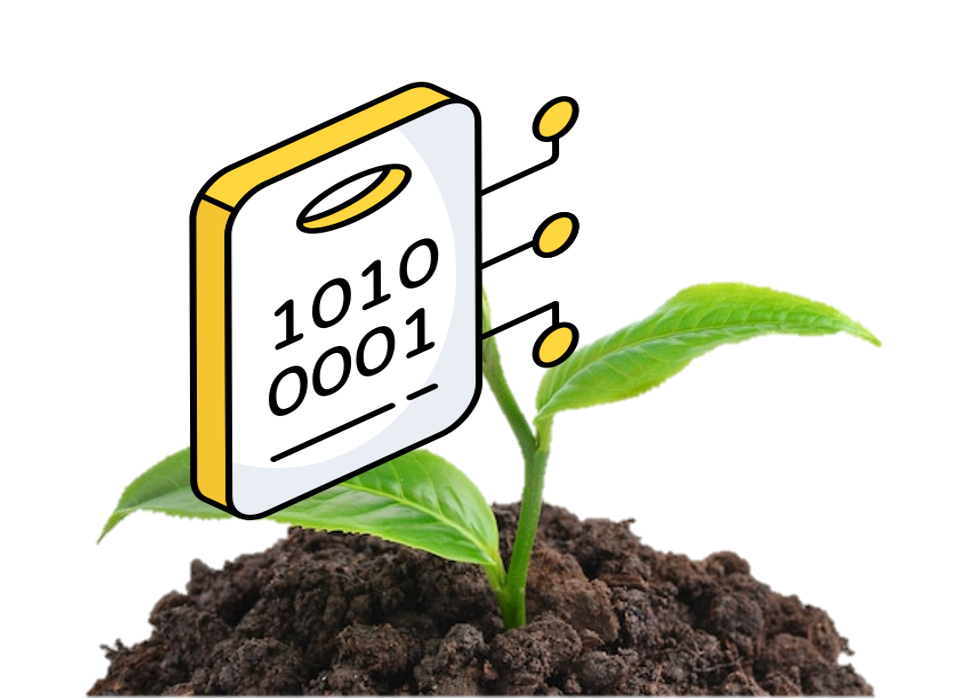
\includegraphics[width=0.4\textwidth]{images/Agrodatascience.png}
\end{frame}


\begin{frame}{Motivación del problemas}
	\begin{block}{\centering Trabajos previos}
		\begin{minipage}{0.5\textwidth}
			Cultivos anuales
			\begin{itemize}
				\item Hortalizas.
			\end{itemize}
		\end{minipage}%
		\begin{minipage}{0.5\textwidth}
			Cultivos perennes
			\begin{itemize}
				\item Árboles frutales.
			\end{itemize}
		\end{minipage}
	\end{block}
	\pause
	\centering\begin{minipage}{0.75\textwidth}
		\begin{block}{\bf Agave}
			\pause\,\,\,Anual\,\, --- Reproducción, trasplantación y {\bf producción}.\\
			\phantom{Perenne --- Inversión económica, rentabilidad y {\bf producción}.} 
		\end{block}
	\end{minipage}

	\,\\
	
	\phantom{\centering \Large  Simultáneamente, anual y perenne.}\\
	\begin{minipage}{0.5\textwidth}
	\vspace{-1.5cm}\raggedright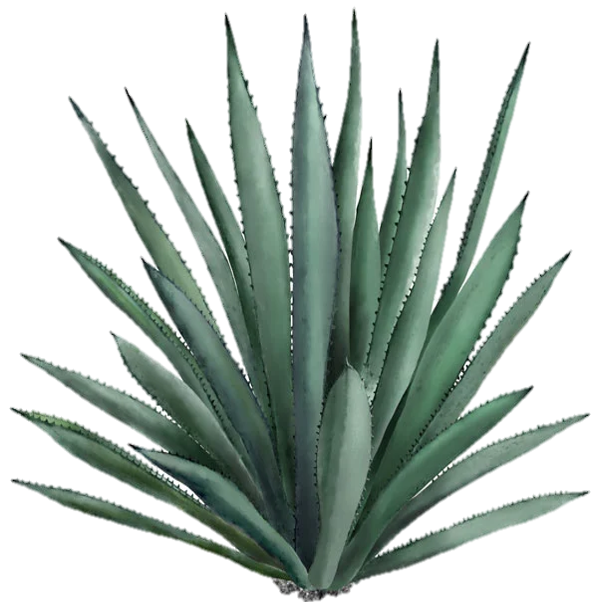
\includegraphics[scale=0.18]{Agave.png}\hfill
\end{minipage}%
\begin{minipage}{0.5\textwidth}
	\phantom{\vspace{-1cm}\raggedleft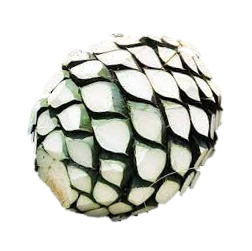
\includegraphics[scale=0.25]{AgavePina.png}}
\end{minipage}
\end{frame}




\begin{frame}{Motivación del problemas}
	\begin{block}{\centering Trabajos previos}
		\begin{minipage}{0.5\textwidth}
			Cultivos anuales
			\begin{itemize}
				\item Hortalizas.
			\end{itemize}
		\end{minipage}%
		\begin{minipage}{0.5\textwidth}
			Cultivos perennes
			\begin{itemize}
				\item Árboles frutales.
			\end{itemize}
		\end{minipage}
	\end{block}
	\centering\begin{minipage}{0.75\textwidth}
	\begin{block}{\bf Agave}
		\,\,\,Anual\,\, --- Reproducción, trasplantación y {\bf producción}.\\
		 Perenne --- Inversión económica, rentabilidad y {\bf producción}. 
	\end{block}
\end{minipage}

\,\\

\phantom{\centering \Large  Simultáneamente, anual y perenne.}\\

\begin{minipage}{0.5\textwidth}
	\vspace{-1.5cm}\raggedright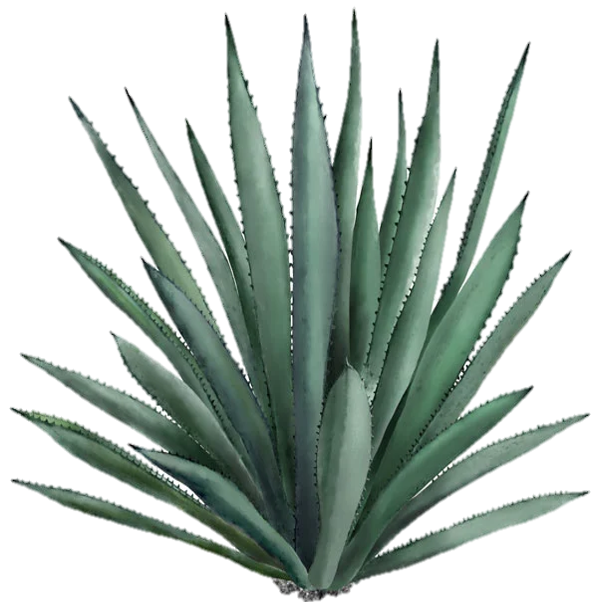
\includegraphics[scale=0.18]{Agave.png}\hfill
\end{minipage}%
\begin{minipage}{0.5\textwidth}
	\vspace{-1cm}\raggedleft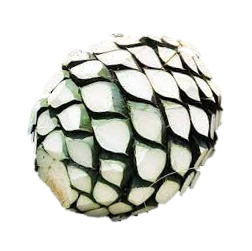
\includegraphics[scale=0.25]{AgavePina.png}
\end{minipage}%
\end{frame}

\begin{frame}{Motivación del problemas}
	\begin{block}{\centering Trabajos previos}
		\begin{minipage}{0.5\textwidth}
			Cultivos anuales
			\begin{itemize}
				\item Hortalizas.
			\end{itemize}
		\end{minipage}%
		\begin{minipage}{0.5\textwidth}
			Cultivos perennes
			\begin{itemize}
				\item Árboles frutales.
			\end{itemize}
		\end{minipage}
	\end{block}
	\centering\begin{minipage}{0.75\textwidth}
		\begin{block}{\bf Agave}
			\,\,\,Anual\,\, --- Reproducción, trasplantación y {\bf producción}.\\
			Perenne --- Inversión económica, rentabilidad y {\bf producción}. 
		\end{block}
	\end{minipage}
	
	\,\\
	
	\centering \Large  Simultáneamente, anual y perenne.\\
	
	\begin{minipage}{0.5\textwidth}
		\vspace{-1.5cm}\raggedright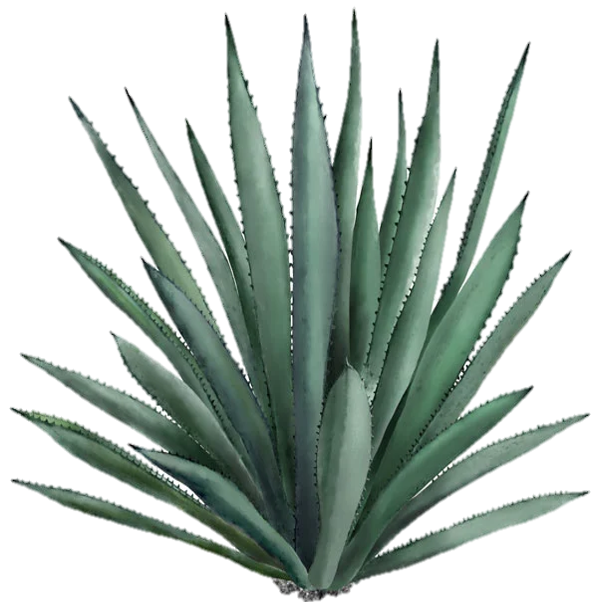
\includegraphics[scale=0.18]{Agave.png}\hfill
	\end{minipage}%
	\begin{minipage}{0.5\textwidth}
		\vspace{-1cm}\raggedleft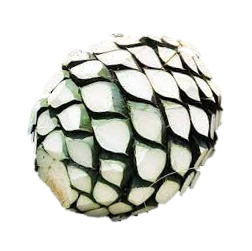
\includegraphics[scale=0.25]{AgavePina.png}
	\end{minipage}%
\end{frame}

\begin{frame}{Industria agrícola}
	\vspace{-1cm}
	\begin{minipage}{0.5\textwidth}
		\begin{block}{Estabilidad}
			\begin{itemize}
				\item Periodo luminoso.
				\item Temperaturas.
				\item Humedad.
				\item Características de suelo.
				\item Polinización.
				
			\end{itemize}
		\end{block}
	\end{minipage}%
	\begin{minipage}{0.5\textwidth}
		\pause\begin{block}{En ausencia}
			\begin{itemize}
				\item Problemas de seguridad alimentaria.
				\item Desequilibrio en la cadena trófica.
				\pause
				\item Desabasto en industrias dependientes.
				\item Problemas económicos.
				\item Conflictos sociales.
			\end{itemize}
		\end{block}
	\end{minipage}
	\pause
	\centering
	\,\\ \Large
	La agricultura es fundamental para un desarrollo integral.
\end{frame}


\begin{frame}{Impacto del cambio climático}
    \vspace{-1.5cm}
    \begin{block}{\centering Alteraciones a largo plazo en los patrones climáticos}
       \begin{minipage}{0.5\textwidth}
			\pause\begin{itemize}
				\item Aumento en las temperaturas.
                \item Aumento de incendios forestales.
			\end{itemize}
		\end{minipage}%
		\pause\begin{minipage}{0.5\textwidth}
			\begin{itemize}
				\item Disponibilidad de agua.
                \item Cambios en los suelos.
			\end{itemize}
		\end{minipage}
    \end{block}

    \begin{minipage}{0.5\textwidth}
			\pause\begin{block}{Factores naturales}
				\begin{itemize}
					\item Actividad solar.
					\item Erupciones volcánicas.
				\end{itemize}
			\end{block}
		\end{minipage}%
		\begin{minipage}{0.5\textwidth}
			\pause\vspace{0cm}\begin{block}{Factores humanos}
				\begin{itemize}
					\item Quema de combustibles fósiles.
					\item Actividad industrial. \phantom{p}
				\end{itemize}
			\end{block}
		\end{minipage}
        \,\\
    \hfill \scriptsize Fuente: ONU (2025).
\end{frame}

\begin{frame}{Impacto del cambio climático}
\vspace{-1cm}

\begin{block}{\centering Consecuencias}
       \begin{minipage}{0.5\textwidth}
			\begin{itemize}
				\item Estrés ambiental.
                \item Relaciones biológicas.
			\end{itemize}
		\end{minipage}%
		\begin{minipage}{0.5\textwidth}
			\begin{itemize}
				\item Escasez laboral.
                \item Volatilidad productiva.
			\end{itemize}
		\end{minipage}
    \end{block}
    \pause
    \begin{block}{Desfase de las estaciones del año \hfill {\scriptsize Fuente: Wang \textit{et al.} (2021).}}
    \centering
        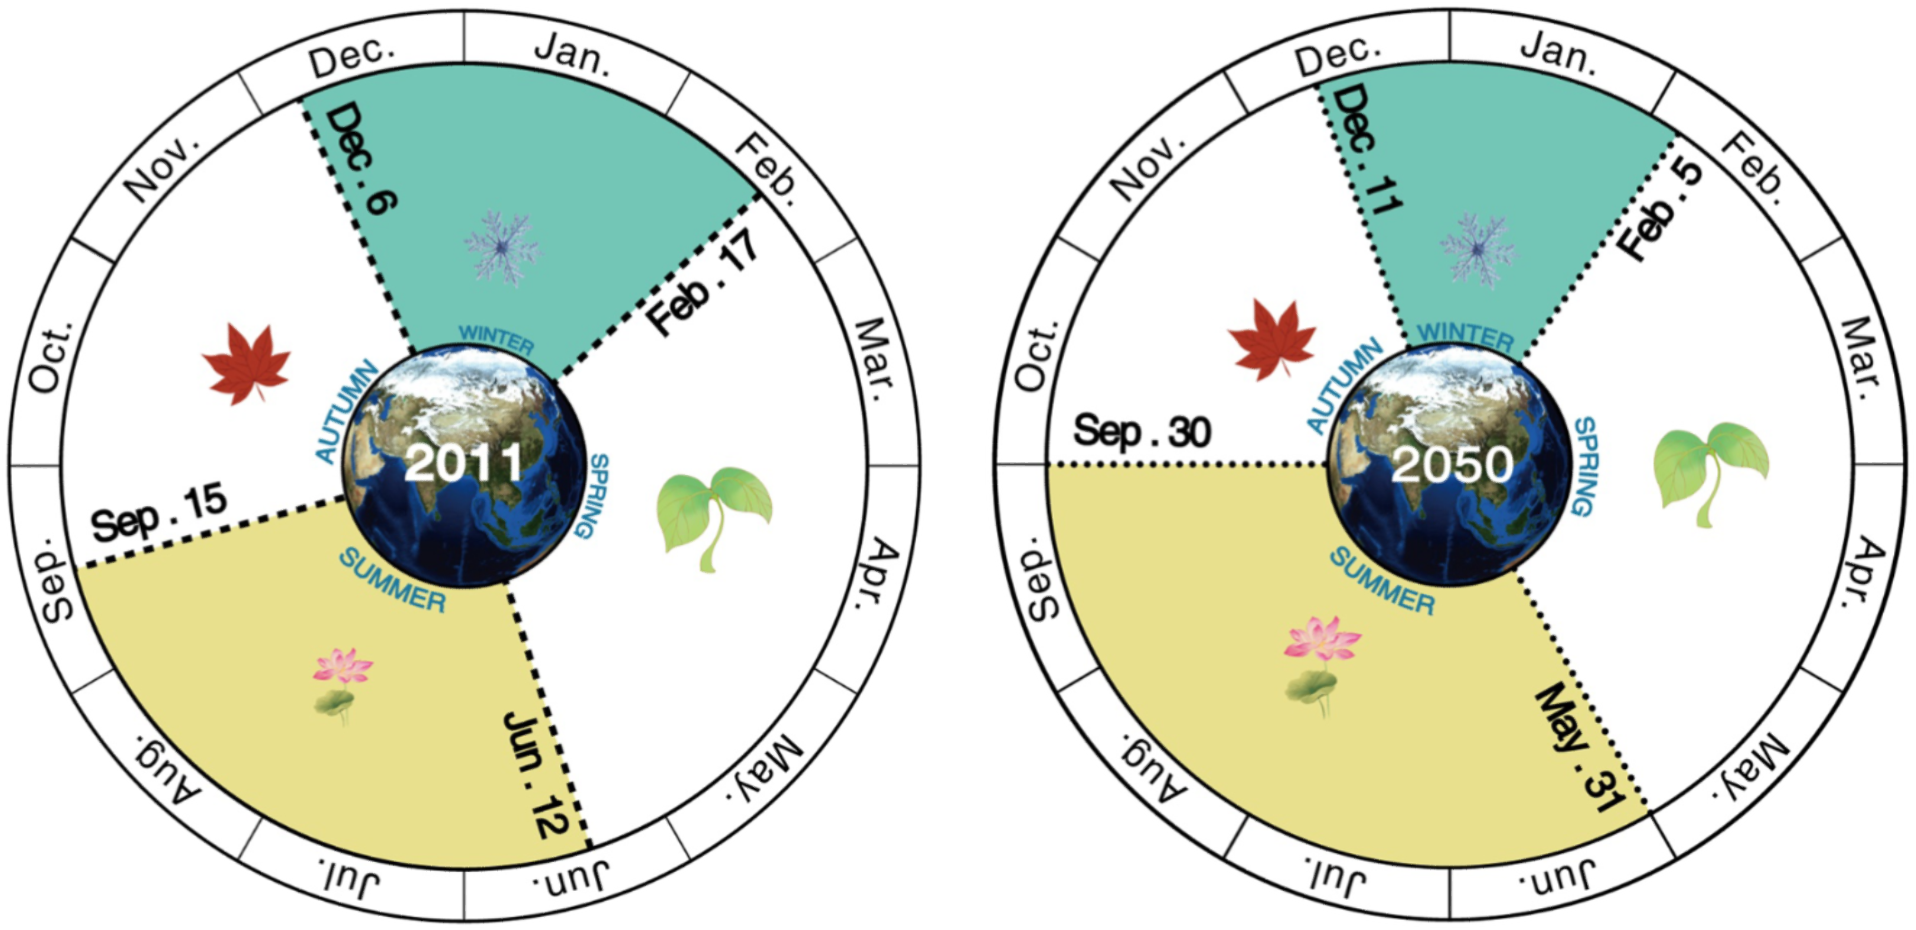
\includegraphics[scale=0.31]{images/Seasons.png}
    \end{block}
\end{frame}


\begin{frame}{El agave}
	\begin{minipage}{0.5\textwidth}
		\centering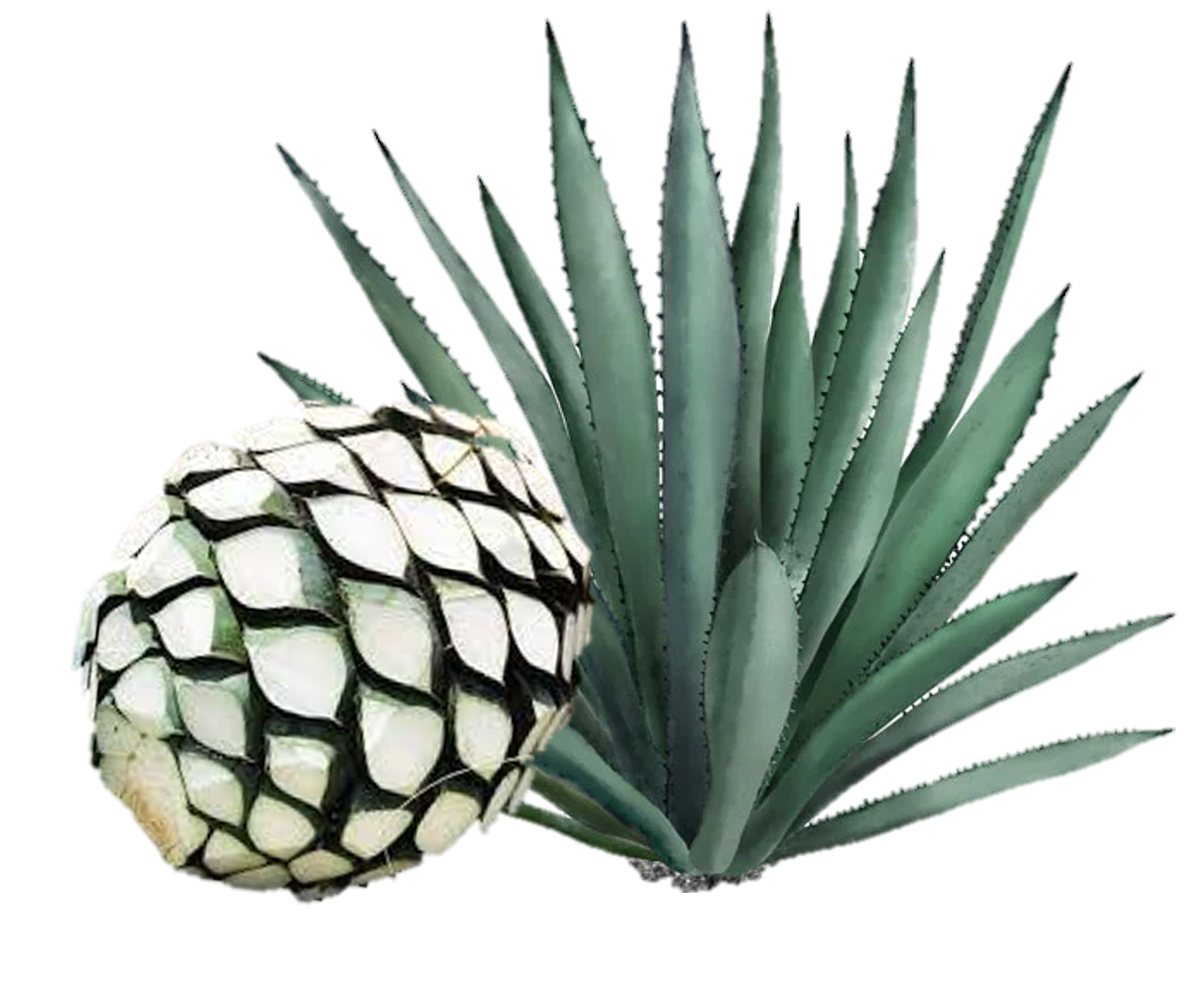
\includegraphics[width=\textwidth]{AgaveyPina.png}
	\end{minipage}%
	\begin{minipage}{0.5\textwidth}
		\begin{block}{}
			\begin{itemize}
				\item Diversidad de especies nativas.
				\item Presencia del 75\% en el territorio nacional.
				\item Aportación del 1.25\% del PIB agrícola.
				\item Tolera altas temperaturas, radiación solar y sequías.
			\end{itemize}
			 {\scriptsize Fuente: García-Mendoza, A. (2007); SAGARPA (2017);  Fernández Galicia \textit{et al.} (2023).}
		\end{block}
	\end{minipage}
	\pause\centering Se especula que será el cultivo más rentable del futuro.\\
	{\scriptsize Fuente: Stewart, J.R. (2015).}
\end{frame}

\begin{frame}{Ciclo productivo}
	\includegraphics[width=\textwidth]{CiclodeProducción.png}\\
	{\scriptsize Fuente: Fernández Galicia \textit{et al.} (2023).}
\end{frame}

\begin{frame}{Ciclo productivo}
	\includegraphics[width=\textwidth]{CiclodeProducción1.png}\\
	{\scriptsize Fuente: Fernández Galicia \textit{et al.} (2023).}
\end{frame}

\begin{frame}{Ciclo productivo}
	\includegraphics[width=\textwidth]{CiclodeProducción2.png}\\
	{\scriptsize Fuente: Fernández Galicia \textit{et al.} (2023).}
\end{frame}

\begin{frame}{Ciclo productivo}
	\includegraphics[width=\textwidth]{CiclodeProducción3.png}\\
	{\scriptsize Fuente: Fernández Galicia \textit{et al.} (2023).}
\end{frame}

\begin{frame}{Ciclo productivo}
	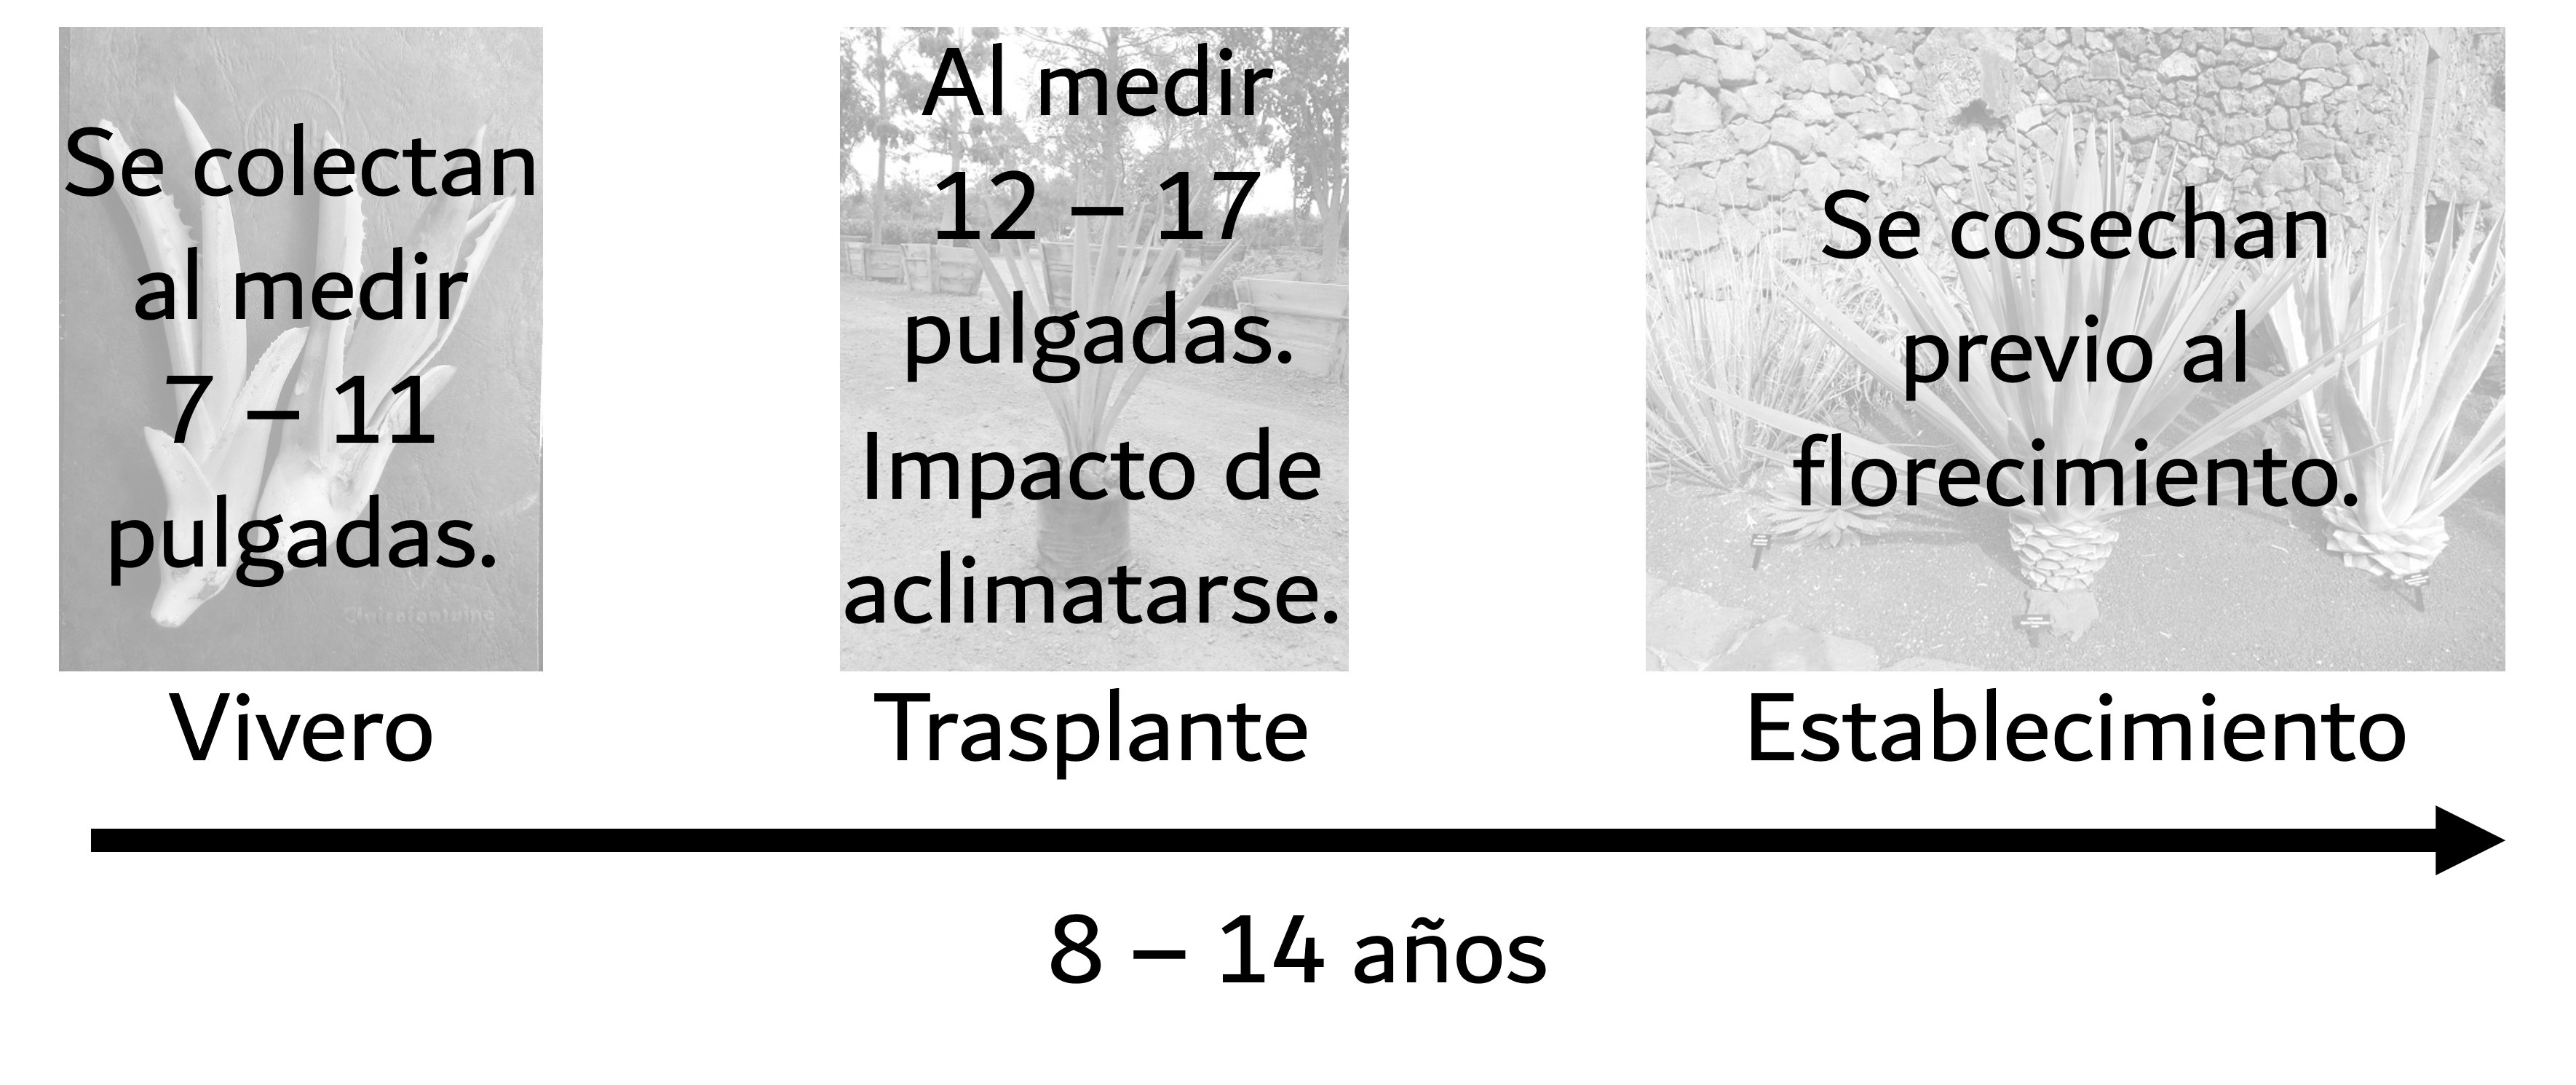
\includegraphics[width=\textwidth]{CiclodeProducción4.png}\\
	{\scriptsize Fuente: Fernández Galicia \textit{et al.} (2023).}
\end{frame}

\begin{frame}{Agave en Aguascalientes}
    \vspace{-1cm}
    \begin{minipage}{0.5\textwidth}
			\hspace{-0.5cm}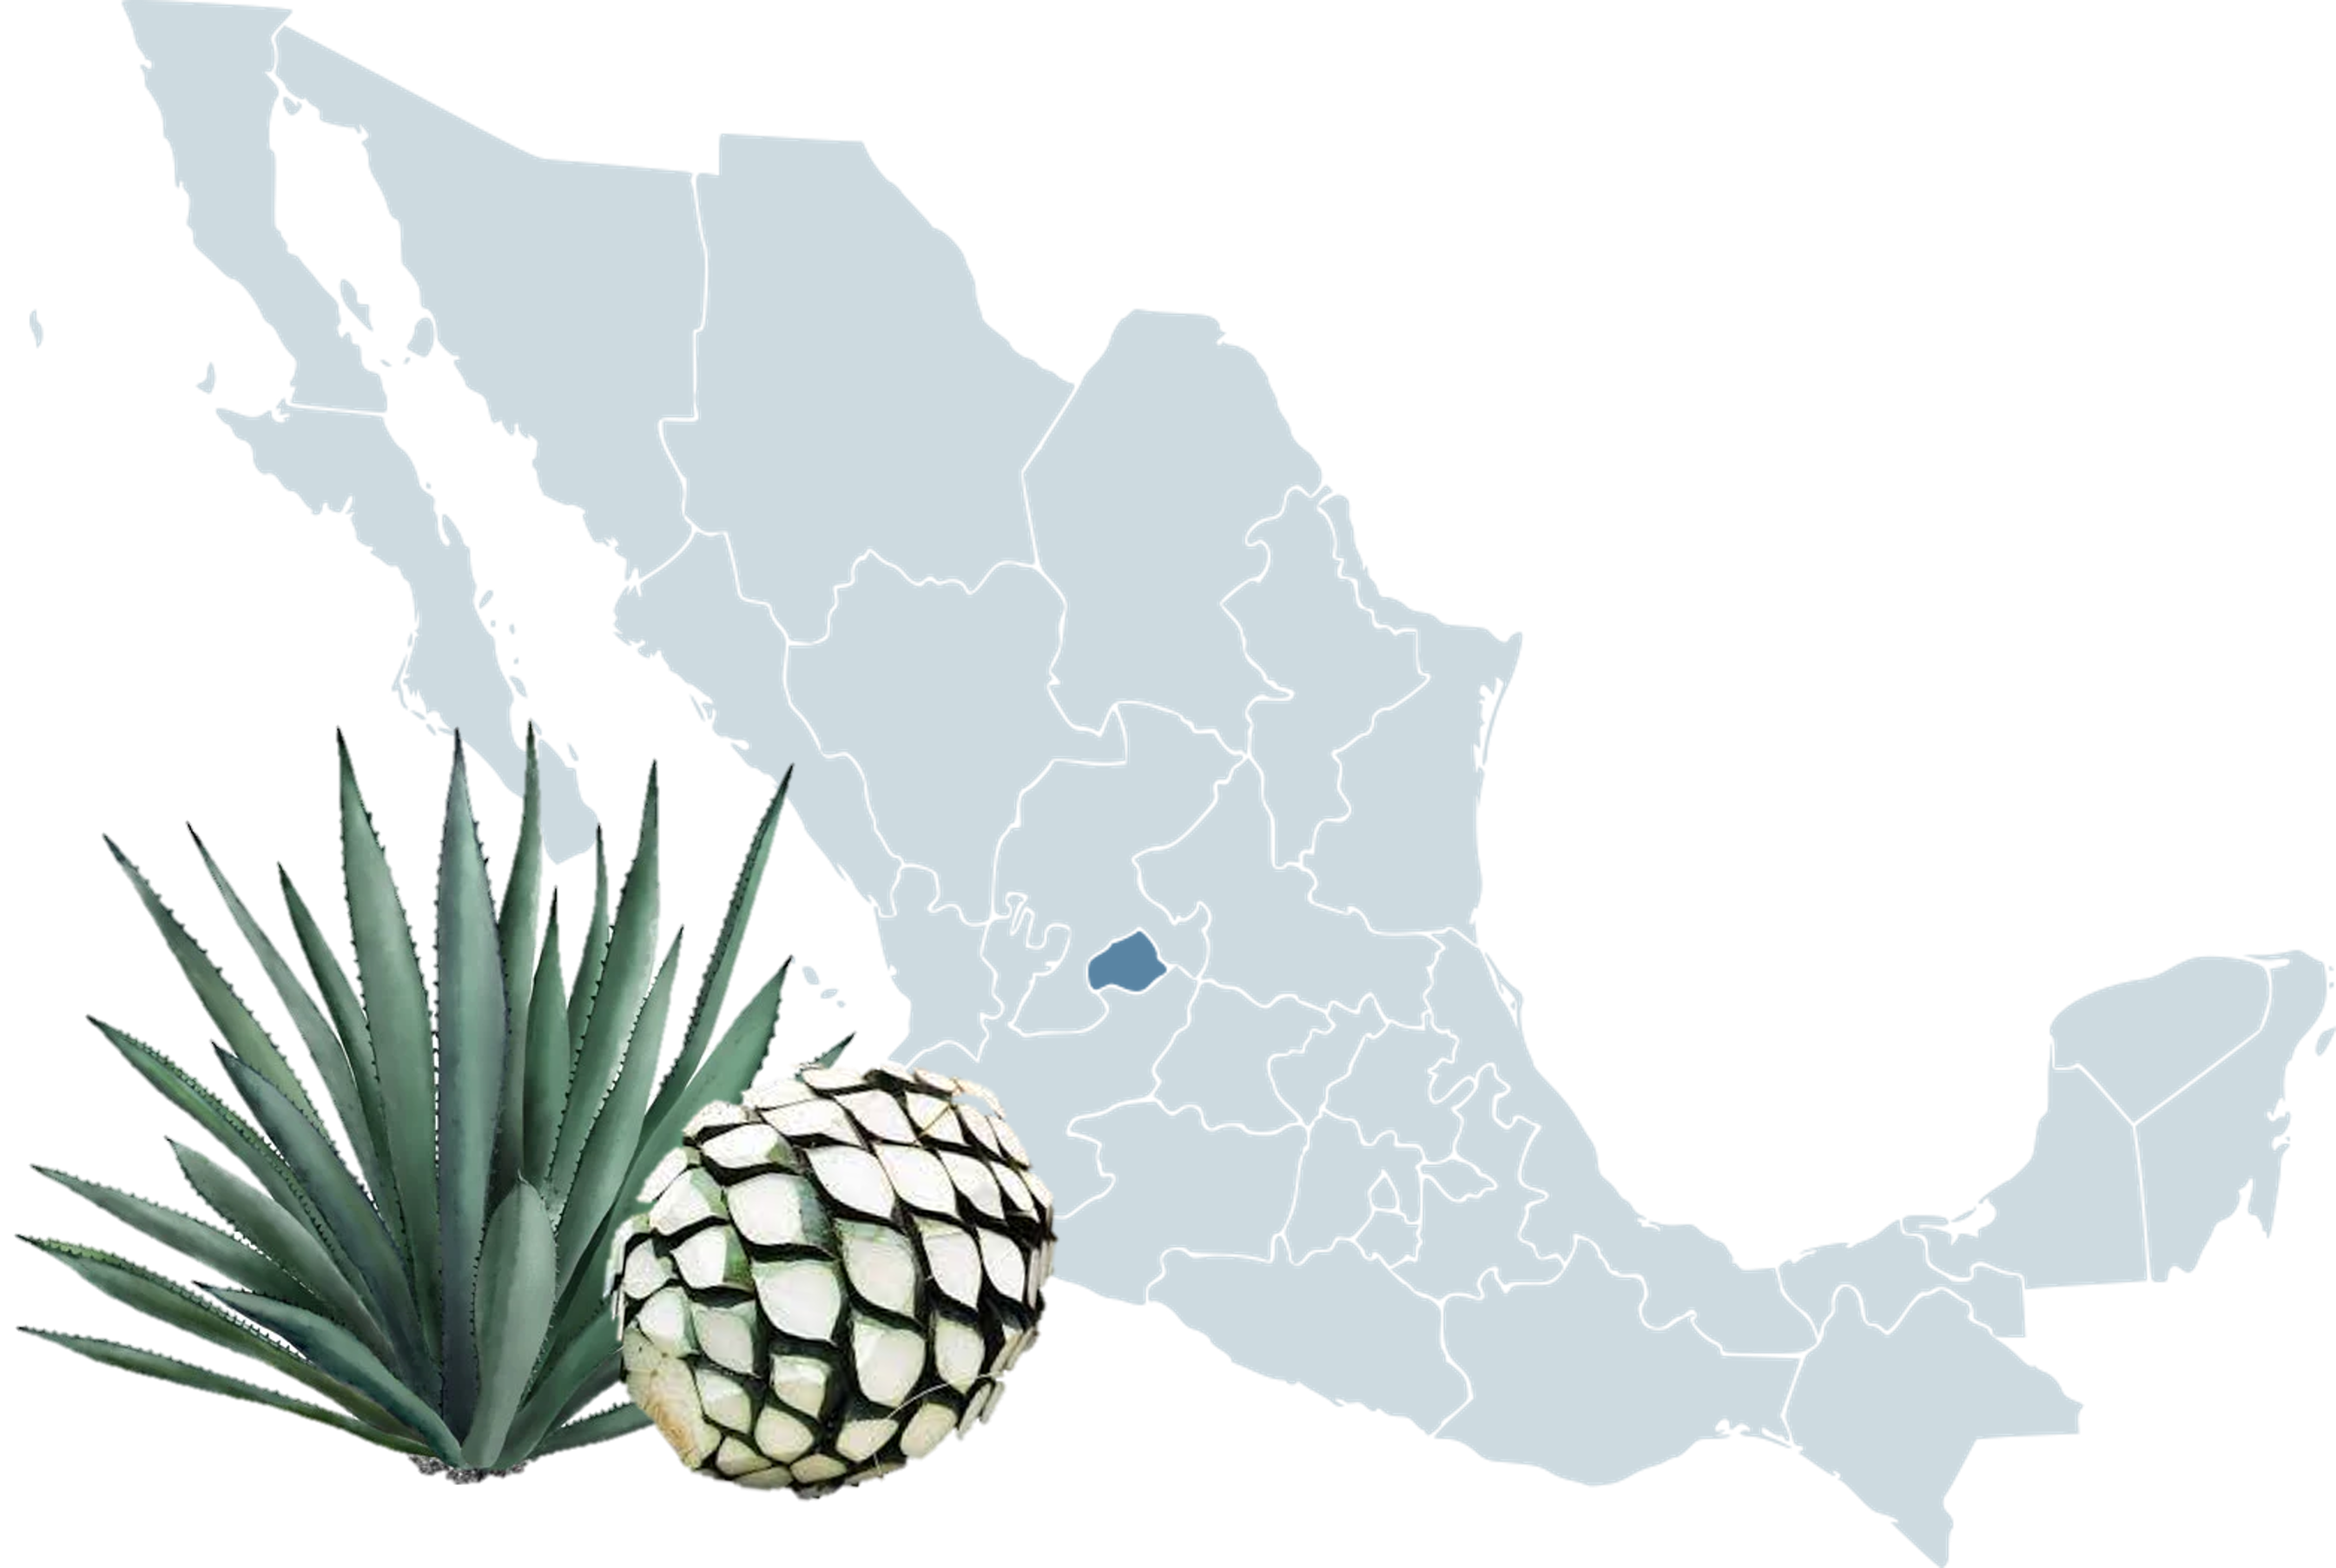
\includegraphics[width=\textwidth]{images/AgaveAGS.png}
		\end{minipage}%
		\begin{minipage}{0.5\textwidth}
			\begin{block}{Angustifolia Haw. y Salmiana Otto ex Salam-Dyck}
				\hfill {\scriptsize Fuente: Gallardo-Valdez \textit{et al.} (2019).}
			\end{block}
            \pause\begin{block}{Requerimientos}
                \begin{itemize}
				\item Suelos con pH de 6 -- 7 y profundidades de, al menos, 1 m.
                    \item Precipitaciones anuales de 600 mm. uniformemente distribuidas.
                    \item Ausencia de heladas.
                    \item Altitudes máximas de 2000 m.s.n.m.
                    \item Temperaturas de -5$^\circ$ C -- 45$^\circ$ C. 
			\end{itemize}
            \end{block}
		\end{minipage}
        \,\\
        \hfill {\scriptsize Fuente: CONAFOR (s.f.);  Fernández Galicia \textit{et al.} (2023).}
\end{frame}


\begin{frame}{Agave en Aguascalientes}
	\vspace{-1cm}
	\begin{minipage}{0.5\textwidth}
		\begin{block}{Productos}
			\begin{itemize}
				\item Bebidas.
				\item Aditivos alimenticios.
				\item Textiles básicos.
				\item Pomadas.
				\item Envases desechables.
			\end{itemize}
			{\scriptsize Fuente: Alonso-Tapia (2022).}
		\end{block}
	\end{minipage}%
	\begin{minipage}{0.5\textwidth}
		\centering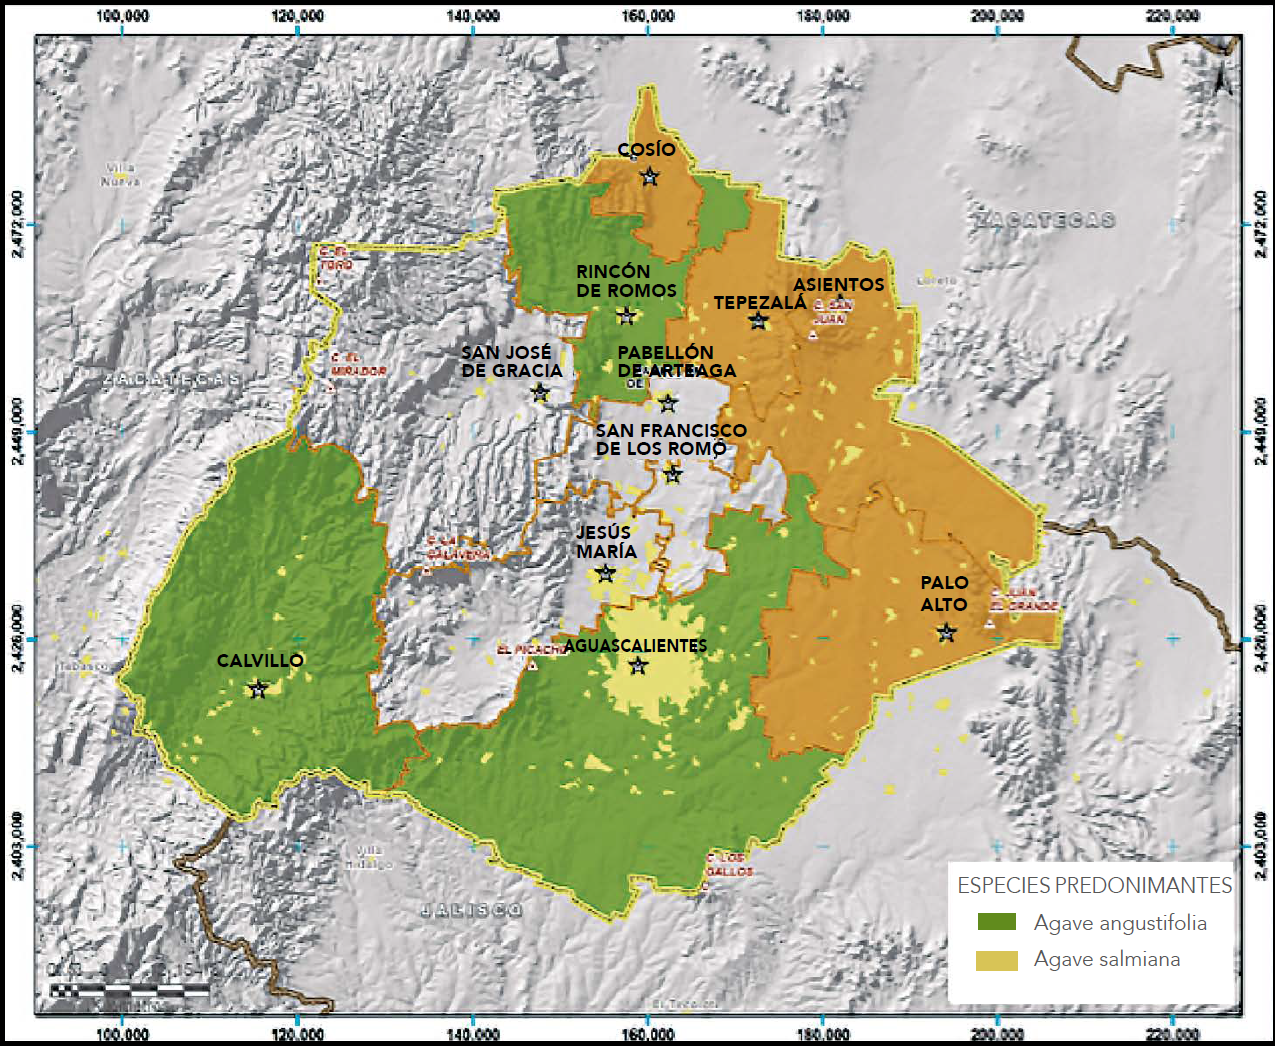
\includegraphics[height=0.73\textheight]{images/DistribucionAGS.png}\\\hfill {\scriptsize Fuente: CIATEJ (2016).}
	\end{minipage}%
\end{frame}


\begin{frame}{Agave en Aguascalientes}
	\vspace{-1cm}
	\begin{minipage}{0.5\textwidth}
		\begin{block}{Usos potenciales}
			\begin{itemize}
				\item Biocombustible.
				\item Bioinsecticidas.
				\item Prebióticos.
				\item Medicamentos.
				\item Textiles complejos.
				\item Papel.
				\item Alimento para animales.
				\item Fitoremediación.
			\end{itemize}
			{\scriptsize Fuente: Stewart, J.R. (2015); Fernández-Galicia, \textit{et al}. (2024).}
		\end{block}
	\end{minipage}%
	\begin{minipage}{0.5\textwidth}
		\centering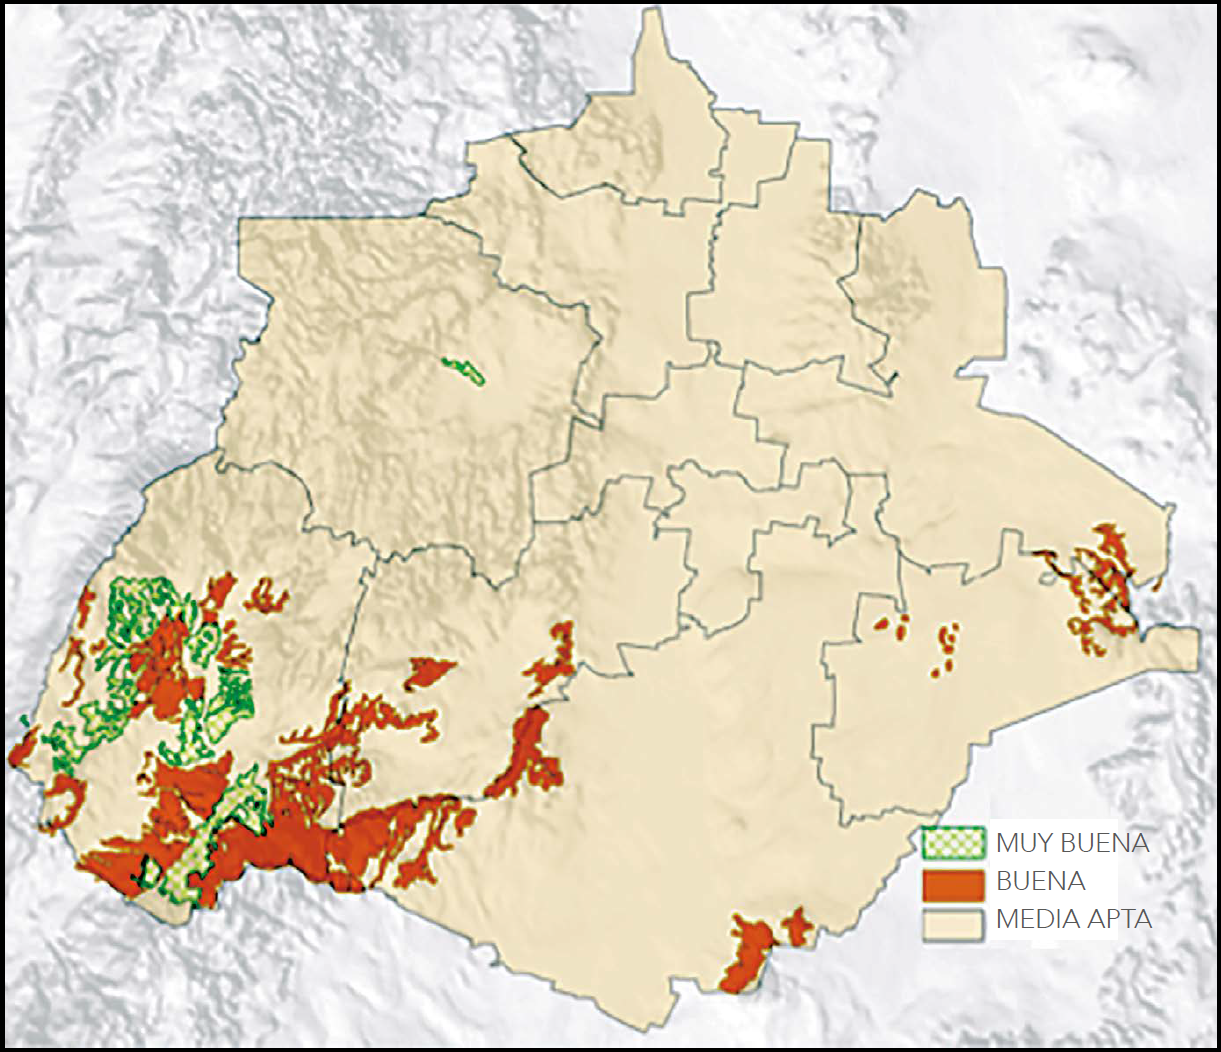
\includegraphics[height=0.73\textheight]{images/AptitudAGS.png}\\\hfill {\scriptsize Fuente: INIFAP (2002).}
	\end{minipage}%
\end{frame}

\begin{frame}{Agave en Aguascalientes}
	\vspace{-1cm}\begin{minipage}{0.5\textwidth}
		\begin{block}{Mezcal con denominación de origen}
			\begin{itemize}
				\item Aguascalientes.
				\item Asientos.
				\item Calvillo.
				\item Cosío.
				\item El Llano.
				\item Rincón de Romos.
				\item Tepezalá.
			\end{itemize}
			{\scriptsize Fuente: IMPI (2025).}
		\end{block}
	\end{minipage}%
\begin{minipage}{0.5\textwidth}
\centering	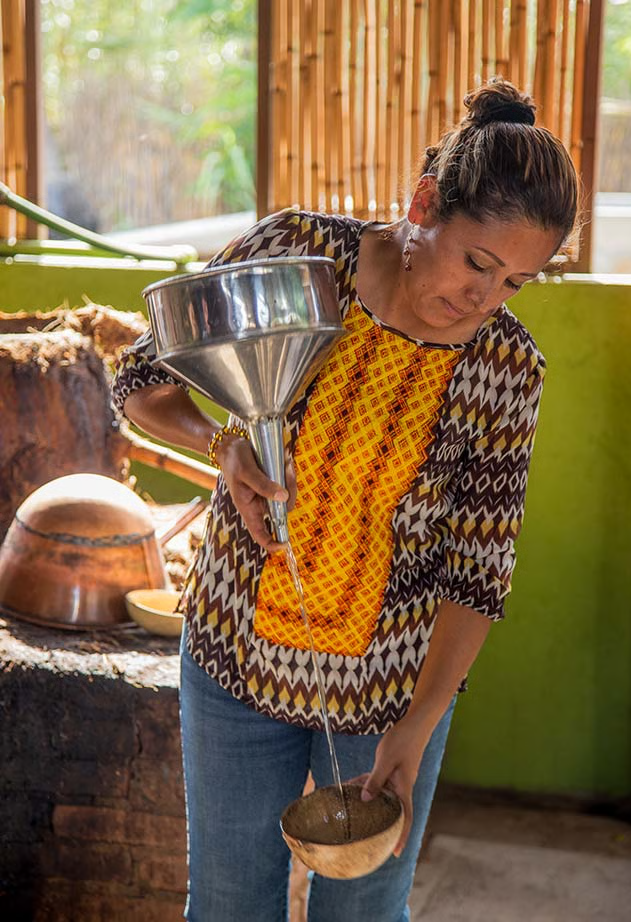
\includegraphics[height=0.7\textheight]{Mezcalera.png}
\end{minipage}
\,\\
\centering \pause El aprovechamiento del agave se encuentra en consolidación.
\end{frame}

\section{Considerando información agroclimática, ¿puede predecirse la evolución del proceso productivo del agave aludiendo a herramientas provenientes de la ciencia de datos?}


\begin{frame}{Objetivos generales}
	\vspace{-1.5cm}Proponer y validar modelos predictivos que permitan: 
	
	\begin{minipage}{0.5\textwidth}
		\pause\begin{block}{Trasplante}
			Determinar periodos ideales.\\ 
			\pause Maximicen tasa de supervivencia.\\
			Reduzcan pérdidas económicas.
		\end{block}
	\end{minipage}%
	\begin{minipage}{0.5\textwidth}\pause\begin{block}{Biomasa\phantom{p}}
			Estimar la producción a escala regional.\\
			\pause Coexistencia de plantas con distintas edades.\phantom{p}
		\end{block}%
	\end{minipage}
	
	\,\\
	\pause
	Lo anterior, empleando información agroclimática relevante para el agave de Aguascalientes, un cultivo que, por su manejo agrícola, puede considerarse simultáneamente anual y perenne.
\end{frame}

\begin{frame}{Estado del arte}
	\vspace{-1cm}\begin{minipage}{0.4\textwidth}
		\begin{block}{Revisión bibliográfica}
			\begin{itemize}
				\item ACM: 100 artículos.
				\item ScienceDirect: 658 artículos.
				\item Kaggle.
				\item UC Irvine.
			\end{itemize}
		\end{block}
	\end{minipage}%
	\pause\begin{minipage}{0.6\textwidth}
		\begin{block}{Trabajos}
			\begin{itemize}
				\item Predecir zonas potenciales.
				\item Segmentación y clasificación de madurez y calidad.
				\item Detección y conteo de plantas.
				\item Contracción de áreas de cultivo.
				\item Densidad de los cultivos.
				\item Viabilidad económica.
				\item Costo económico del trasplante manual y mecanizado.
				\pause\item \bf Estimación de biomasa fresca y seca.
				\pause\item \sout{Fechas de trasplante.}
			\end{itemize}
		\end{block}
	\end{minipage}%
\end{frame}

\begin{frame}{Estado del arte: Estimación individual}
	\begin{minipage}{0.5\textwidth}
		\begin{block}{Peso seco}
			\begin{itemize}
				\item López-Díaz, \textit{et al.} (2022): Regresión de la forma $Y=\beta_0 X^{\beta_1}\varepsilon$.\\
				Diámetro de la corona como variable explicativa.
				\item Vuorinne, \textit{et al.} (2021): Regresión lineal para biomasa de hojas.\\
				Anchura máxima y altura como variable explicativa.
			\end{itemize}
		\end{block}
	\end{minipage}%
	\begin{minipage}{0.5\textwidth}
		\begin{block}{Peso fresco}
			\begin{itemize}
				\item López Serrano, \textit{et al.} (2022): Regresión de la forma $Y=\beta_0 X^{\beta_1}\varepsilon$.\\
				Diámetro de la corona como variable explicativa.
				\item Velazco-Baustista, \textit{et al.} (2009): Regresión bivariada.\\
				Diámetro de la roseta y altura de la planta como variables explicativas.
			\end{itemize}
		\end{block}
	\end{minipage}
\end{frame}

\begin{frame}{Estado del arte: Estimación colectiva}
	\begin{minipage}{0.5\textwidth}
		\begin{block}{Peso seco}
			\begin{itemize}
				\item Vuorinne, \textit{et al.} (2021): Integran análisis de imágenes provenientes del Sentinel-2 para extender la cobertura de sus estimaciones.
			\end{itemize}
		\end{block}
	\end{minipage}%
	\begin{minipage}{0.5\textwidth}
		\begin{block}{}
			Nobel, P.S. (1984): Propone el índice de productividad ambiental (EPI).
			\begin{itemize}
				\item Índice mensual de agua.
				\item Índice mensual de temperatura.
				\item Índice mensual de radiación fotosintéticamente activa. 
			\end{itemize}
			Al ponderarlo con la absorción de CO$_2$ por unidad de área estima la producción.
		\end{block}
	\end{minipage}
\end{frame}

\begin{frame}{Factibilidad: Estimación de la producción}
	  \begin{minipage}{0.6\textwidth}
	  	\vspace{-1cm}\begin{block}{}
	  		\begin{itemize}
	  			\item Akin \textit{et al.} (2017): Modelo de suavizamiento exponencial de Brown genera un pronóstico a 10 años para la producción de aguacate en Turquía.
	  		\end{itemize}
	  			\phantom{.}\\
	  			\phantom{.}\\
	  			\phantom{.}\\
	  			\phantom{.}\\
	  			\phantom{.}\\
	  			\phantom{.}\\
	  	\end{block}
	  \end{minipage}%
	  \begin{minipage}{0.4\textwidth}
	  	\vspace{-0.5cm}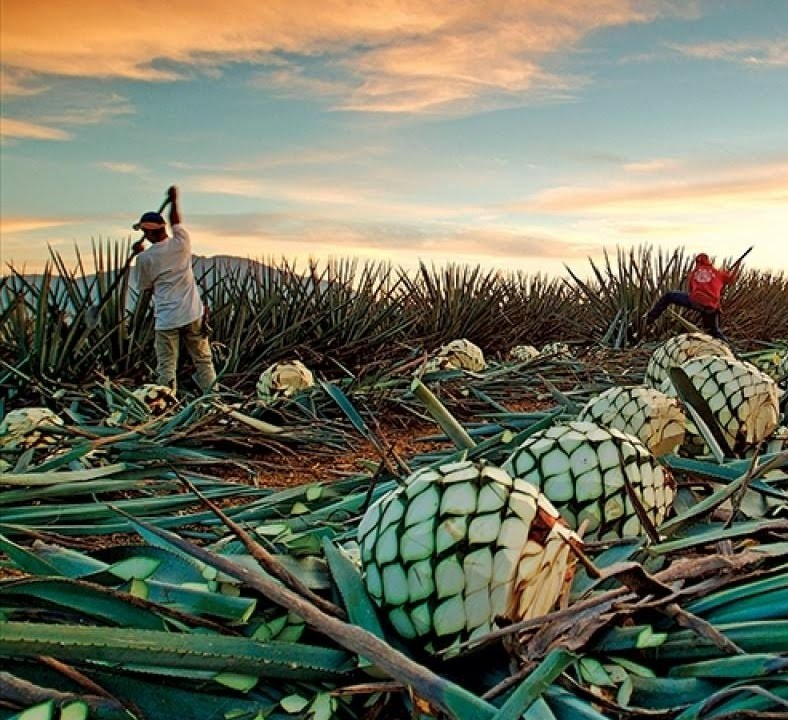
\includegraphics[scale=0.3]{Biomass.jpg}
	  \end{minipage}%
\end{frame}

\begin{frame}{Factibilidad: Estimación de la producción}
	\begin{minipage}{0.6\textwidth}
		\vspace{-1cm}\begin{block}{}
			\begin{itemize}
				\item Akin \textit{et al.} (2017): Modelo de suavizamiento exponencial de Brown genera un pronóstico a 10 años para la producción de aguacate en Turquía.
				\item Arizmendi-Peralta, P.P. (2024): Propone al algoritmo Random Forest Regressor como mejor estimador para estimar la producción de aguacate en una hectárea.
				\item Mosquera \textit{et al.} (2015): Estima la producción de huertas de aguacates, de la misma edad, a través de un modelo de regresión cuadrático.
			\end{itemize}
		\end{block}
	\end{minipage}%
	\begin{minipage}{0.4\textwidth}
		\vspace{-0.5cm}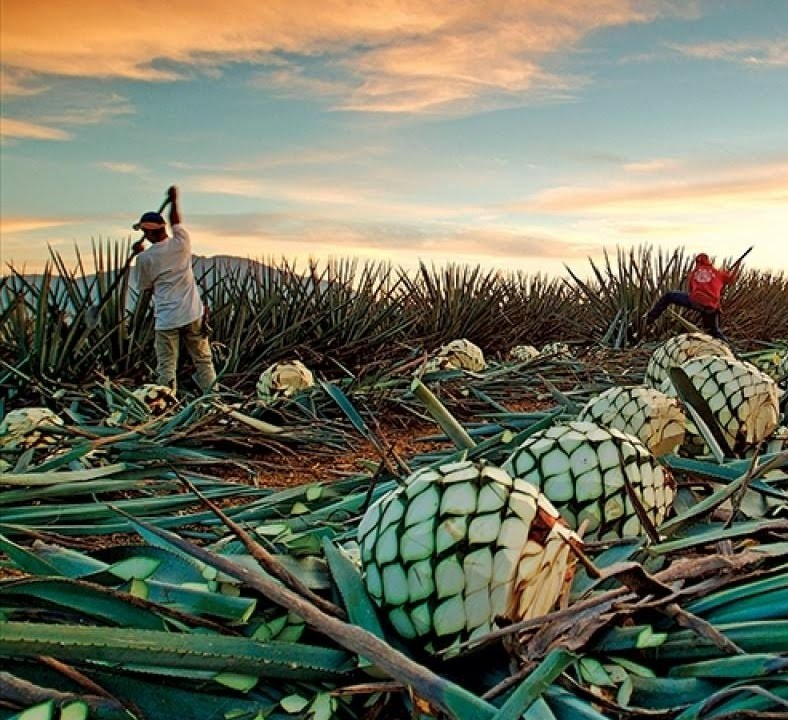
\includegraphics[scale=0.3]{Biomass.jpg}
	\end{minipage}%
\end{frame}

\begin{frame}{Factibilidad: Fechas de trasplante}
	\begin{minipage}{0.5\textwidth}
		\hspace{-0.5cm}
		\centering
		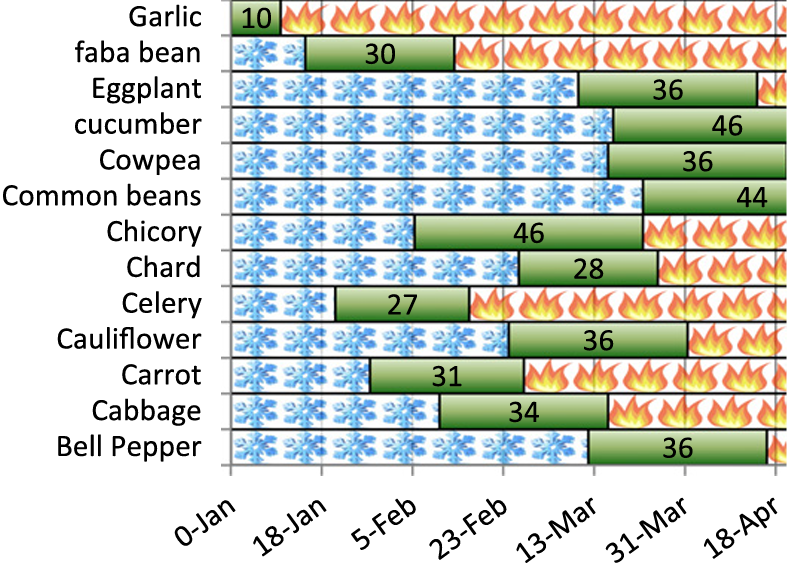
\includegraphics[width=\textwidth]{images/Elnesr.png}
		{\scriptsize Fuente: Elnesr \textit{et al.} (2013).}
	\end{minipage}%
	\begin{minipage}{0.5\textwidth}
		\begin{block}{}
			\begin{itemize}
				\item Elnesr \textit{et al.} (2013): Propone un algoritmo determinista de decisión simple.
				\item Dobor \textit{et al.} (2016): Implementa el modelo determinista M4 para obtener fechas para el trigo.
				\item Gümüşçü \textit{et al.} (2018): Emplea modelos de ML aplicados al trigo.
			\end{itemize}
		\end{block}
	\end{minipage}
\end{frame}

\begin{frame}{Factibilidad: Fechas de trasplante}
	\begin{minipage}{0.5\textwidth}
		\begin{block}{}
			\begin{itemize}
				\item Boechel \textit{et al.} (2022): Implementa modelos de ML para la cosecha de manzanas.
				\item Fakhrzad \textit{et al.} (2025): Emplea modelos de ML aplicados al árbol de jamaica.
			\end{itemize}
		\end{block}
	\end{minipage}%
	\begin{minipage}{0.5\textwidth}
		\hspace{-0.5cm}
		\centering
		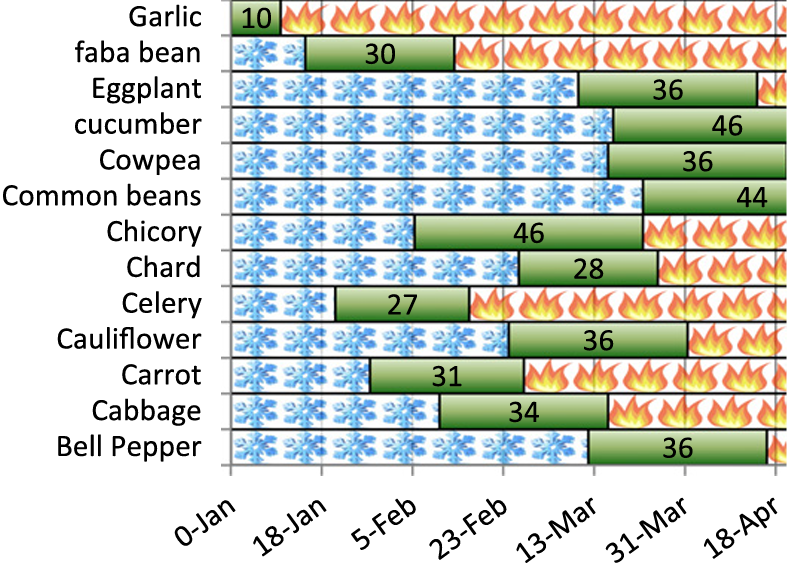
\includegraphics[width=\textwidth]{images/Elnesr.png}
		{\scriptsize Fuente: Elnesr \textit{et al.} (2013).}
	\end{minipage}%
\end{frame}




\begin{frame}{Datos disponibles}
    \vspace{-1cm}
    \begin{minipage}{0.5\textwidth}
			\hspace{-0.5cm}
            \centering
            
\includegraphics[width=\textwidth]{images/Essenger.png}
		\end{minipage}%
		\begin{minipage}{0.5\textwidth}
            \begin{block}{}
                \begin{itemize}
                    \item Instituto Nacional de Investigaciones Forestales, Agrícolas y Pecuarias.
				\item Registros diarios de estaciones climáticas.
                    \item Periodo de enero de 1980 a diciembre de 2022.
                    \item Temperatura del aire.
                    \item Periodo luminoso.
                    \item Radiación de onda corta.
                    \item Lluvia líquida.
                    \item Presión de vapor.
			\end{itemize}
            \end{block}
		\end{minipage}
\end{frame}
\begin{frame}{Datos disponibles}
    \vspace{-1cm}
		\begin{minipage}{0.5\textwidth}
            \begin{block}{}
                \begin{itemize}
                    \item INIFAP.
				\item Datos medidos en diversas profundidades.
                    \item Rango de 0 a 200 cm.
                    \item Porción de limo.
                    \item Capacidad de intercambio catiónico.
                    \item Nitrógeno.
                    \item Carbono orgánico.
                    \item pH.
			\end{itemize}
            \end{block}
		\end{minipage}%
        \begin{minipage}{0.5\textwidth}
			\hspace{0cm}
            \centering
            
\includegraphics[width=\textwidth]{images/MSMx.png}
		\end{minipage}
\end{frame}

\begin{frame}{Datos disponibles}
    \vspace{-1cm}
    \begin{minipage}{0.5\textwidth}
			\hspace{-0.5cm}
            \centering
            
\includegraphics[width=\textwidth]{images/conagua.png}
		\end{minipage}%
		\begin{minipage}{0.5\textwidth}
            \begin{block}{}
                \begin{itemize}
                    \item Sistema Meteorológico Nacional.
				\item Registros diarios a nivel estatal.
                    \item Periodo de enero de 1960 a abril de 2025.
                    \item Temperatura ambiental.
                    \item Evaporación.
                    \item Precipitación.
                    \item Lluvia líquida.
			\end{itemize}
            \end{block}
		\end{minipage}
\end{frame}



\section*{Referencias}
\begin{frame}[allowframebreaks,noframenumbering]{Referencias}
	\vspace*{-1cm}
	\tiny
	\bibliography{Bibliografia.bib}
	\bibliographystyle{alpha}
	\nocite{*}
	%\printbibliography
\end{frame}

\section*{Gracias}
\begin{frame}[noframenumbering]
%\vspace{2cm}
     \begin{center}
	    \Huge{Gracias}
	\end{center}
    \end{frame}
    
    
 \begin{frame}{}
 	 \begin{block}{Métodos}
 		\begin{itemize}
 			\item Algoritmos de decisión simple.
 			\item Modelos de suavizamiento exponencial.
 			\item Redes neuronales recurrentes.
 			\item Regresiones.
 			\item Perceptrón multicapa.
 			\item Support vector machine.
 			\item Árboles de decisión.
 			\item Bosques aleatorios.
 			\item k vecinos más cercanos.
 			\item M5 Prime.
 		\end{itemize}
 	\end{block}
 \end{frame}
\end{document}
